% !TEX root = diss.tex

\chapter{Do non-redox active metal cations have the potentials to behave as
chemo-protective agents? The Effects on Metal Cations on HAT Reaction Barrier
Heights} \label{ch:hat}

\begin{doublespace}
\section{Introduction}

Metal cations are ubiquitous in biological systems and play an important role in
biological function. As such, there is a great deal of interest in studying
metals in biological systems. Proteins in particular are often associated with
metals, and in the worldwide Protein Data Bank,\cite{Harding2010, Berman2007}
over one-third of crystal structures contain metals. Redox active metals, such
as copper and iron, act as co-factors in metalloenzymes for important catalytic
processes.\cite{Atkins2010}

Non-redox active metal cations are equally as important in biological function
as redox active metals, where they are essential to protein structure and
function, along with cellular and neuronal signalling.\cite{Karp1999} Sodium and
calcium ions are most abundant extracellularly, while potassium and magnesium
are dominant inside of cells. Specific ionic concentrations vary dramatically
depending on physiological conditions; estimates for equilibrium concentrations
in both mammalian heart cells\cite{Ingwall2006} and blood
plasma\cite{daSilva2001} are listed in~\ref{tab:metalconc}. As sodium and
magnesium are the most abundant alkali and alkaline earth metals found in
biologically relevant systems, they are of prime interest for my investigation.

\begin{table}[!htbp]
  \caption[Ionic concentrations inside a mammalian heart cell and in the blood
  plasma.]{Ionic concentrations inside a mammalian heart cell and in the blood
  plasma. Concentrations are in units of mM. Values are rounded to one
  significant figure. Data are from Ref. \protect\citenum{Ingwall2006} and
  \protect\citenum{daSilva2001}.} \label{tab:metalconc}
\begin{tabular}{l c c}
  Ion Conc. & Mammalian Cells & Blood Plasma \\
  \hline
  \ch{Na^+} & 10 & 100--200 \\
  \ch{Mg^{2+}} & 10 & 1 \\
  \ch{K^+} & 100 & 4 \\
  \ch{Ca^{2+}} & 0.1 & 2
\end{tabular}
\end{table}

Extensive crystallographic surveys indicate that metals bind predominantly to
oxygen centres in proteins.\cite{Harding1999, Harding2004, Hsin2008} Divalent
metals are most often found bound directly to proteins. Calcium binds anywhere
from 4 to 6 binding sites in protein crystal structures, while magnesium binds
only 1 or 2. Monovalent metals, on the other hand, are often heavily solvated
and so they appear in solvent cavities of proteins, although sodium or potassium
are sometimes found bound directly to carbonyl or carboxylate oxygen
centres.\cite{Harding2010}

A great deal of research has focussed on \ch{Ca^{2+}} in the context of reactive
oxygen-centred radical production.\cite{Goerlach2015} Specifically, \ch{Ca^{2+}}
ions are important in the mitochondria, where, depending on physiological
conditions and concentrations, they can act as inhibitors or promoters of
free-radical production in the electron transport chain.\cite{AdamVizi2010} One
explanation is that \ch{Ca^{2+}} induce conformational changes of the proteins
involved in the electron transport chain that are responsible for radical
generation.\cite{Brookes2004} Mitochondrial free-radicals, when present in
moderate amounts, can act as cell signalling molecules to activate pro-growth
responses.\cite{Sullivan2014} However, ``dysfunctional'' mitochondria can
produce excess radicals leading to oxidative damage that has been linked to
degenerative diseases.

Given the significant importance alkali and alkaline earth metals play in
biological systems, their impact on protein oxidation must be considered.
However, until recently, kinetic studies of protein oxidation have not
investigated the mechanistic role of non-redox active metals. In a series of
three papers,\cite{Salamone2013a, Salamone2015metals, Salamone2016} Bietti and
colleagues showed that alkali and alkaline earth metals have an inhibitory
effect on HAT reactions involving \cumo\ and organic substrates. Some of the
experimental rate constants from these papers are summarized
in~\ref{tab:hat-metals}. All rate constants were obtained by time-resolved LFP
in nitrogen or argon-saturated acetonitrile (MeCN) at 298 K, as was previously
described in Section~\ref{sec:hat-methods}. The experimental results have been
rationalized on the basis of Lewis acidic metal cation interactions with Lewis
basic substrates.


\begin{table}
  \caption{Summary of rate constants for reactions of \cumo\ with various
  organic substrates in the presence of alkali and alkaline earth metal salts.}
  \label{tab:hat-metals}
  \hspace*{-0.6cm}
  \begin{tabular}{l l c c}
    Substrate & Conditions & $k_H$ (\Ms) & $k_H$(MeCN)/$k_H$(M$^{n+}$) \\
    \hline
    1,4-cyclohexadiene &    & 6.7\E{7} & \\
    (CHD)  & \ch{LiClO4} 1.0 M & 7.5\E{7} & 0.89 \\
     & \ch{Mg(ClO4)2} 1.0 M & 7.0\E{7} & 0.96 \\
    tetrahydrofuran &   & 5.7\E{6} & \\
    (THF) & \ch{LiClO4} 1.0 M & 2.9\E{6} & 1.7 \\
     & \ch{LiOTf} 1.0 M & 2.8\E{6} & 2.0 \\
     & \ch{Mg(ClO4)2} 1.0 M & 1.8\E{6} & 3.2 \\
    triethylamine &  & 2.0\E{8} & \\
    (TEA) & \ch{LiClO4} 1.0 M & 9.4\E{7} & 2.1 \\
     & \ch{Mg(ClO4)2} 0.005 M & $<$1\E{6} & $>$200 \\
    $N,N$-dimethylformamide & & 1.2\E{6} & \\
    (DMF) & \ch{LiClO4} 0.5 M & $k_{H1}$ = 8.9\E{5} & 1.3 \\
      & & $k_{H2}$ = 1.5\E{6} & 0.80 \\
      & \ch{NaClO4} 0.2 M & $k_{H1}$ = 9.6\E{5} & 1.3 \\
      & & $k_{H2}$ = 1.4\E{6} & 0.86 \\
      & \ch{Mg(ClO4)2} 0.2 M & $k_{H1}$ = 5.8\E{5} & 2.1 \\
      & & $k_{H2}$ = 1.1\E{6} & 1.1 \\
      & \ch{Ca(ClO4)2} 0.2 M & $k_{H1}$ = 1.0\E{6} & 0.83 \\
    $N,N$-dimethylacetamide &  & 1.2\E{6} & \\
    (DMA) & \ch{LiClO4} 0.2 M & $k_{H1}$ = 8.5\E{5} & 1.4 \\
      & & $k_{H2}$ = 1.5\E{6} & 0.8 \\
      & \ch{NaClO4} 0.2 M & $k_{H1}$ = 1.1\E{6} & 1.1 \\
      & & $k_{H2}$ = 1.3\E{6} & 0.92 \\
      & \ch{Mg(ClO4)2} 0.2 M & $k_{H1}$ = 4.7\E{5} & 2.6 \\
      & & $k_{H2}$ = 2.4\E{5} & 5.0 \\
      & & $k_{H3}$ = 1.1\E{6} & 1.1 \\
      & \ch{Ca(ClO4)2} 0.2 M & $k_{H1}$ = 1.2\E{6} & 1.0
  \end{tabular}
\end{table}

For hydrocarbons, cyclic ethers, and tertiary amines, rate constants for
hydrogen abstraction by \cumo\ in the presence of excess concentrations of
lithium and magnesium salts were measured.\cite{Salamone2013a} In the presence
of \ch{LiClO4} and \ch{Mg(ClO4)2}, the rate of abstraction by \cumo\ from
1,4-cyclohexadiene (CHD) increases very slightly. Since CHD has no Lewis basic
centres, the increase in HAT rate constant was explained on the basis of metal
cation interactions with \cumo, very slightly increasing the hydrogen
abstraction ability by withdrawing electron density from the aromatic ring.
Metal cations were also shown to increase the unimolecular decay of \cumo\ by
$\beta$-scission (See Section~\ref{sec:hat-methods}). The largest kinetic effect
was observed with \ch{LiClO4} with $k_\beta$ = 1.8\E{6} $s^{-1}$, which is a
roughly 3-fold increase as compared to the rate in MeCN at 298 K ($k_\beta$ =
6.3\E{5} $s^{-1}$).\cite{Avila1995} This effect is significantly less than the
observed kinetic solvent effect on \cumo\ $\beta$-scission measured in \ch{H2O}
or 2,2,2-trifluoroethanol ($k_\beta$ = 1.0\E{7} and 6.1\E{6} $s^{-1}$,
respectively).\cite{Bietti2005, Neta1984} Therefore, the kinetic effects of
these alkali and alkaline metal salts interacting via Lewis acid-base
interactions with the oxygen-centre of \cumo\ are less than the effects of
hydrogen-bonding by solvents.

Next, the HAT rate constants for abstraction from tetrahydrofuran (THF) decrease
in the presence of non-redox active metal salts. Both \ch{LiClO4} and \ch{LiOTf}
decrease $k_H$ by a factor of about 2, indicating the nature of the
counter-anion plays a negligible role in the Lewis acid-base interactions
between metal cations and substrates. The addition of \ch{Mg(ClO4)2} has a
greater effect on HAT reactivity, decreasing $k_H$ by a factor of 3. The
magnesium ion is a stronger Lewis acid than lithium,\cite{Fukuzumi2002}
supporting the notion of Lewis acid-base interactions between the oxygen
lone-pair and the metal cations. The decrease in $k_H$ has been partially
attributed to the reduction in electron density in the \ch{C-H} $\sigma^*$
anti-bonding orbital which is normally present due to hyperconjugative overlap
with the neighbouring oxygen lone-pair (See~\ref{fig:THF}), as a consequence of
the metal cation withdrawing electron density from the oxygen lone-pair.

A 2-fold decrease in $k_H$ for the tertiary amine, triethylamine (TEA), is
observed upon the addition of \ch{LiClO4}, for which an analogous orbital
interaction explanation is also appropriate. Interestingly, the addition of 1.0
M \ch{Mg(ClO4)2} was reported to immediately form a precipitate. This
precipitate was identified as the formation of a strong TEA-\ch{Mg^{2+}} Lewis
acid-base adduct. This observation is once again consistent with the stronger
Lewis acidity of \ch{Mg^{2+}} as compared to \ch{Li^+}, and also the
significantly greater Lewis basicity of TEA vs THF.\cite{Salamone2013a,
Reichardt2010} It was also pointed out that MeCN will competitively bind with
metal cations, however it is a weaker Lewis base than both THF and TEA.
Measurements of $k_H$ for HAT between \cumo\ and TEA in the presence of 0.005 M
\ch{Mg(ClO4)2} were successful only up until [TEA] = 9.6 mM, at which point a
precipitate began to form. Nonetheless, an upper limit to the hydrogen
abstraction rate constant was estimated as $k_H <$ 1\E{6} \Ms, or at least a 200
fold decrease relative to no metal salt. Very similar results for bulkier
tertiary amines were also obtained. Thus, the addition of strong Lewis acids in
the presence of Lewis basic sites on hydrogen atom donors can deactivate
\ch{C-H} bonds.

Next, we turn to the more relevant models for the work of this thesis, the
tertiary amides $N,N$-dimethylformamide (DMF) and $N,N$-dimethylacetamide (DMA).
As with THF, normal hyperconjugative overlap between the conjugated amide
$\pi$-system and the adjacent \ch{C-H} $\sigma^*$ anti-bonding orbitals weakens
the \ch{C-H} bonds. Therefore, metal binding to the amide oxygen-centre should
result in a decrease in this orbital interaction, strengthen the \ch{C-H} bonds,
and decrease HAT reactivity. In their study, \citet{Salamone2015metals} measured
\cumo\ abstraction rate constants from DMF and DMA in the presence of
stoichiometric equivalents of \ch{LiClO4}, \ch{LiOTf}, \ch{NaClO4},
\ch{Mg(ClO4)2}, and \ch{Ca(ClO4)2} (in contrast to the excess used in
Reference~\citenum{Salamone2013a}). \ref{fig:k-metals-mg}a,b shows the plots of
$k_{obs}$ against [substrate] for the reactions of \cumo\ with DMF and DMA in
MeCN containing 0.2 M \ch{Mg(ClO4)2}, respectively. For both DMF and DMA, there
are three distinct regions in the plots: weak \ch{C-H} bond activation for
[amide]/[\ch{Mg^{2+}}]$\leq 2$, followed by strong \ch{C-H} bond deactivation
for 2$<$[amide]/[\ch{Mg^{2+}}]$\leq$4, and no deactivation for
[amide]/[\ch{Mg^{2+}}]$<$4.

\begin{figure}[!htbp]
  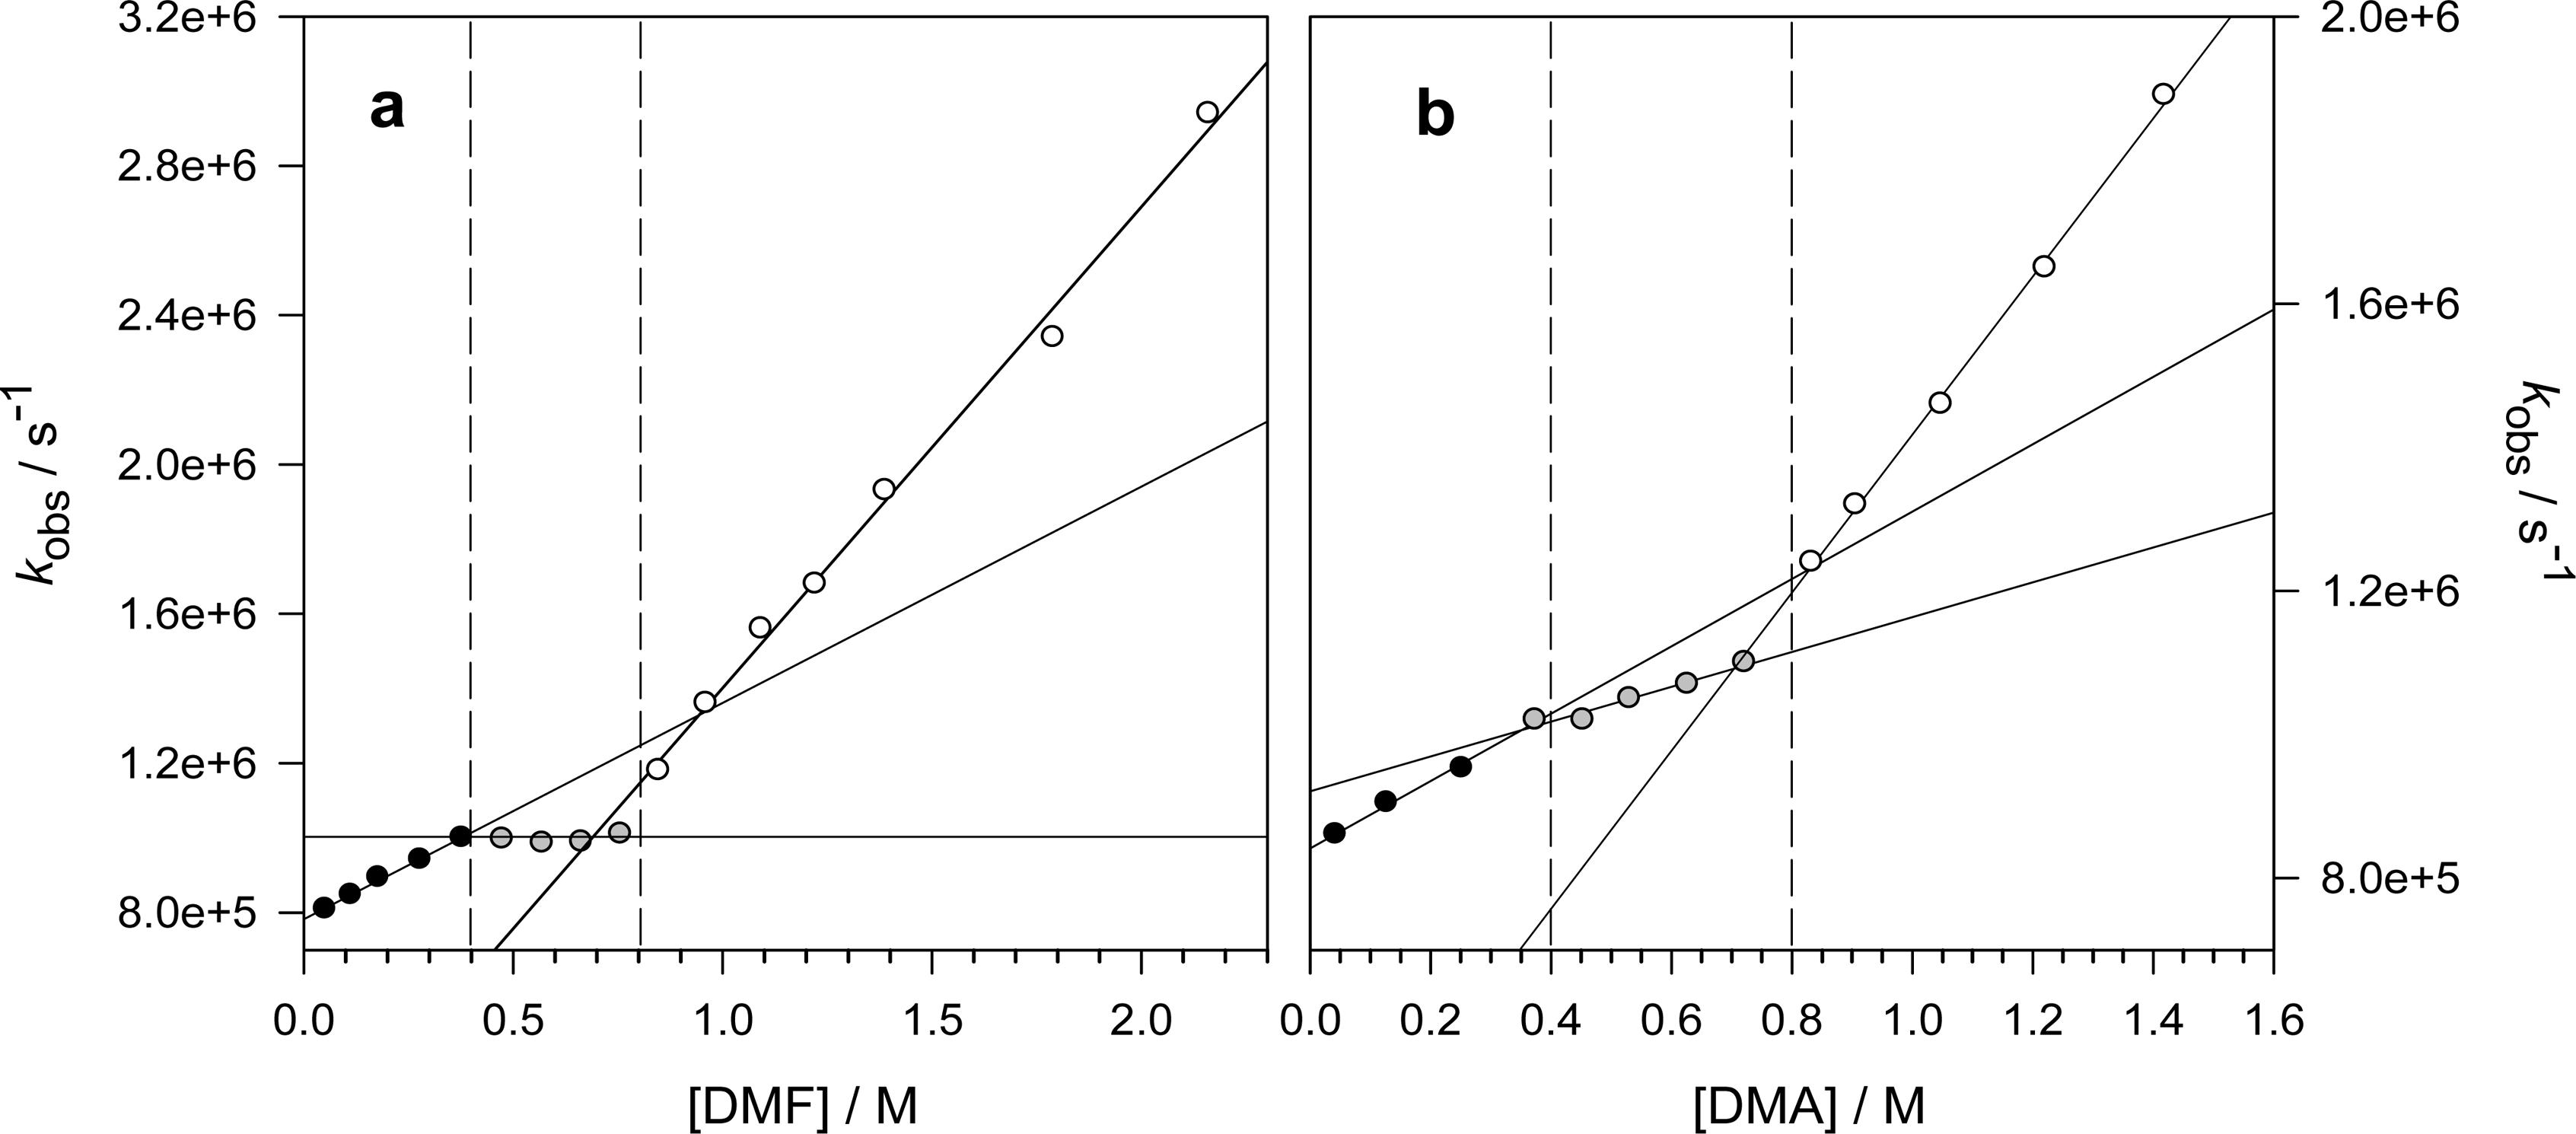
\includegraphics[width=\textwidth]{figures/kH-dma-dmf-mgclo42.png}
  \caption[Plot of observed rate constant against concentration of DMF and DMA
  for reaction with \cumo\ at 298 K in the presence of 0.2 M \ch{Mg(ClO4)2}.]
  {\textbf{a)} Plot of observed rate constant against concentration of DMF for
	  reaction with \cumo\ at 298 K in the presence of 0.2 M
	  \ch{Mg(ClO4)2}. 0--0.4 M [DMF] range (black circles), $k_{H1}$ =
	  5.8\E{5} \Ms; 0.8--2.2 M [DMF] range (white circles), $k_{H2}$ =
	  1.3\E{6} \Ms.  \textbf{b)} Plot of observed rate constant against
  concentration of DMA for reaction with \cumo\ at 298 K in the presence of 0.2
  M \ch{Mg(ClO4)2}. 0--0.4 M [DMA] range (black circles), $k_{H1}$ = 4.7\E{5}
  \Ms; 0.4--0.8 M [DMA] range (grey circles), $k_{H2}$ = 2.4\E{5} \Ms; 0.8--2.2
  M [DMA] range (white circles), $k_{H3}$ = 1.1\E{6} \Ms. Reprinted with
  permission from Reference~\protect\citenum{Salamone2015metals}. Copyright
  2015 American Chemical Society.} \label{fig:k-metals-mg}
\end{figure}

The addition of both \ch{LiClO4} and \ch{LiOTf} decrease to a similar extent the
rate constants for abstraction from DMF and DMA by \cumo. However, in contrast
to \ch{Mg(ClO4)2}, the lithium salts strongly deactivate \ch{C-H} bonds for 2
equivalents, followed by weak deactivation for another 2 equivalents, and no
deactivation for [amide]/[\ch{Li^{+}}]$<$4. Salamone et al. were not able to
give a clear cut explanation, but suggest that the different patterns are a
result of differences in charge density, which is greater for \ch{Mg^{2+}} than
\ch{Li^+}, as well as different coordination geometries of the two ions. A
coordination number of 4 is most common for \ch{Li^+}, while an octahedral
geometry with the coordination of 6 ligands is almost always observed for
\ch{Mg^{2+}}.\cite{Babu2013, Dudev2014} As a result, interactions of the ions
with solvent and counter-anions were suggested to be more important for
\ch{Mg^{2+}} than \ch{Li^+}.

\ch{NaClO4} and \ch{Ca(ClO4)2} influence HAT between \cumo\ and DMA to different
extents than both \ch{LiClO4} and \ch{Mg(ClO4)2}. \ref{fig:k-metals-naca}a,b
shows the plots of $k_{obs}$ against [substrate] for the reactions of \cumo\
with DMA in MeCN containing 0.2 M \ch{NaClO4} and \ch{Mg(ClO4)2}, respectively.
For \ch{NaClO4}, an almost negligible deactivation of \ch{C-H} bonds is observed
for up to 4 equivalents of DMA. This was explained on the basis of the weaker
Lewis acidity of \ch{Na^+} as compared to \ch{Li^+}. With regards to
\ch{Ca(ClO4)2}, binding to DMA fully deactivates \ch{C-H} bond abstraction up to
4 equivalents of DMA. The first region of~\ref{fig:k-metals-naca}b ([DMA] =
0--0.2 M, black circles) represents the decrease in $k_\beta$ of \cumo\ as
\ch{Ca^{2+}} preferentially binds to DMA over \cumo. Interestingly, for both DMF
and DMA, the same experiments in dimethyl sulfoxide (DMSO) solvent show no
inhibition of HAT reactivity by metal cations. This was rationalized on the
basis of the stronger Lewis basicity of DMSO as compared to both MeCN and the
amides, thus the metals preferentially bind the solvent rather than amide
substrate.

\begin{figure}[!htbp]
  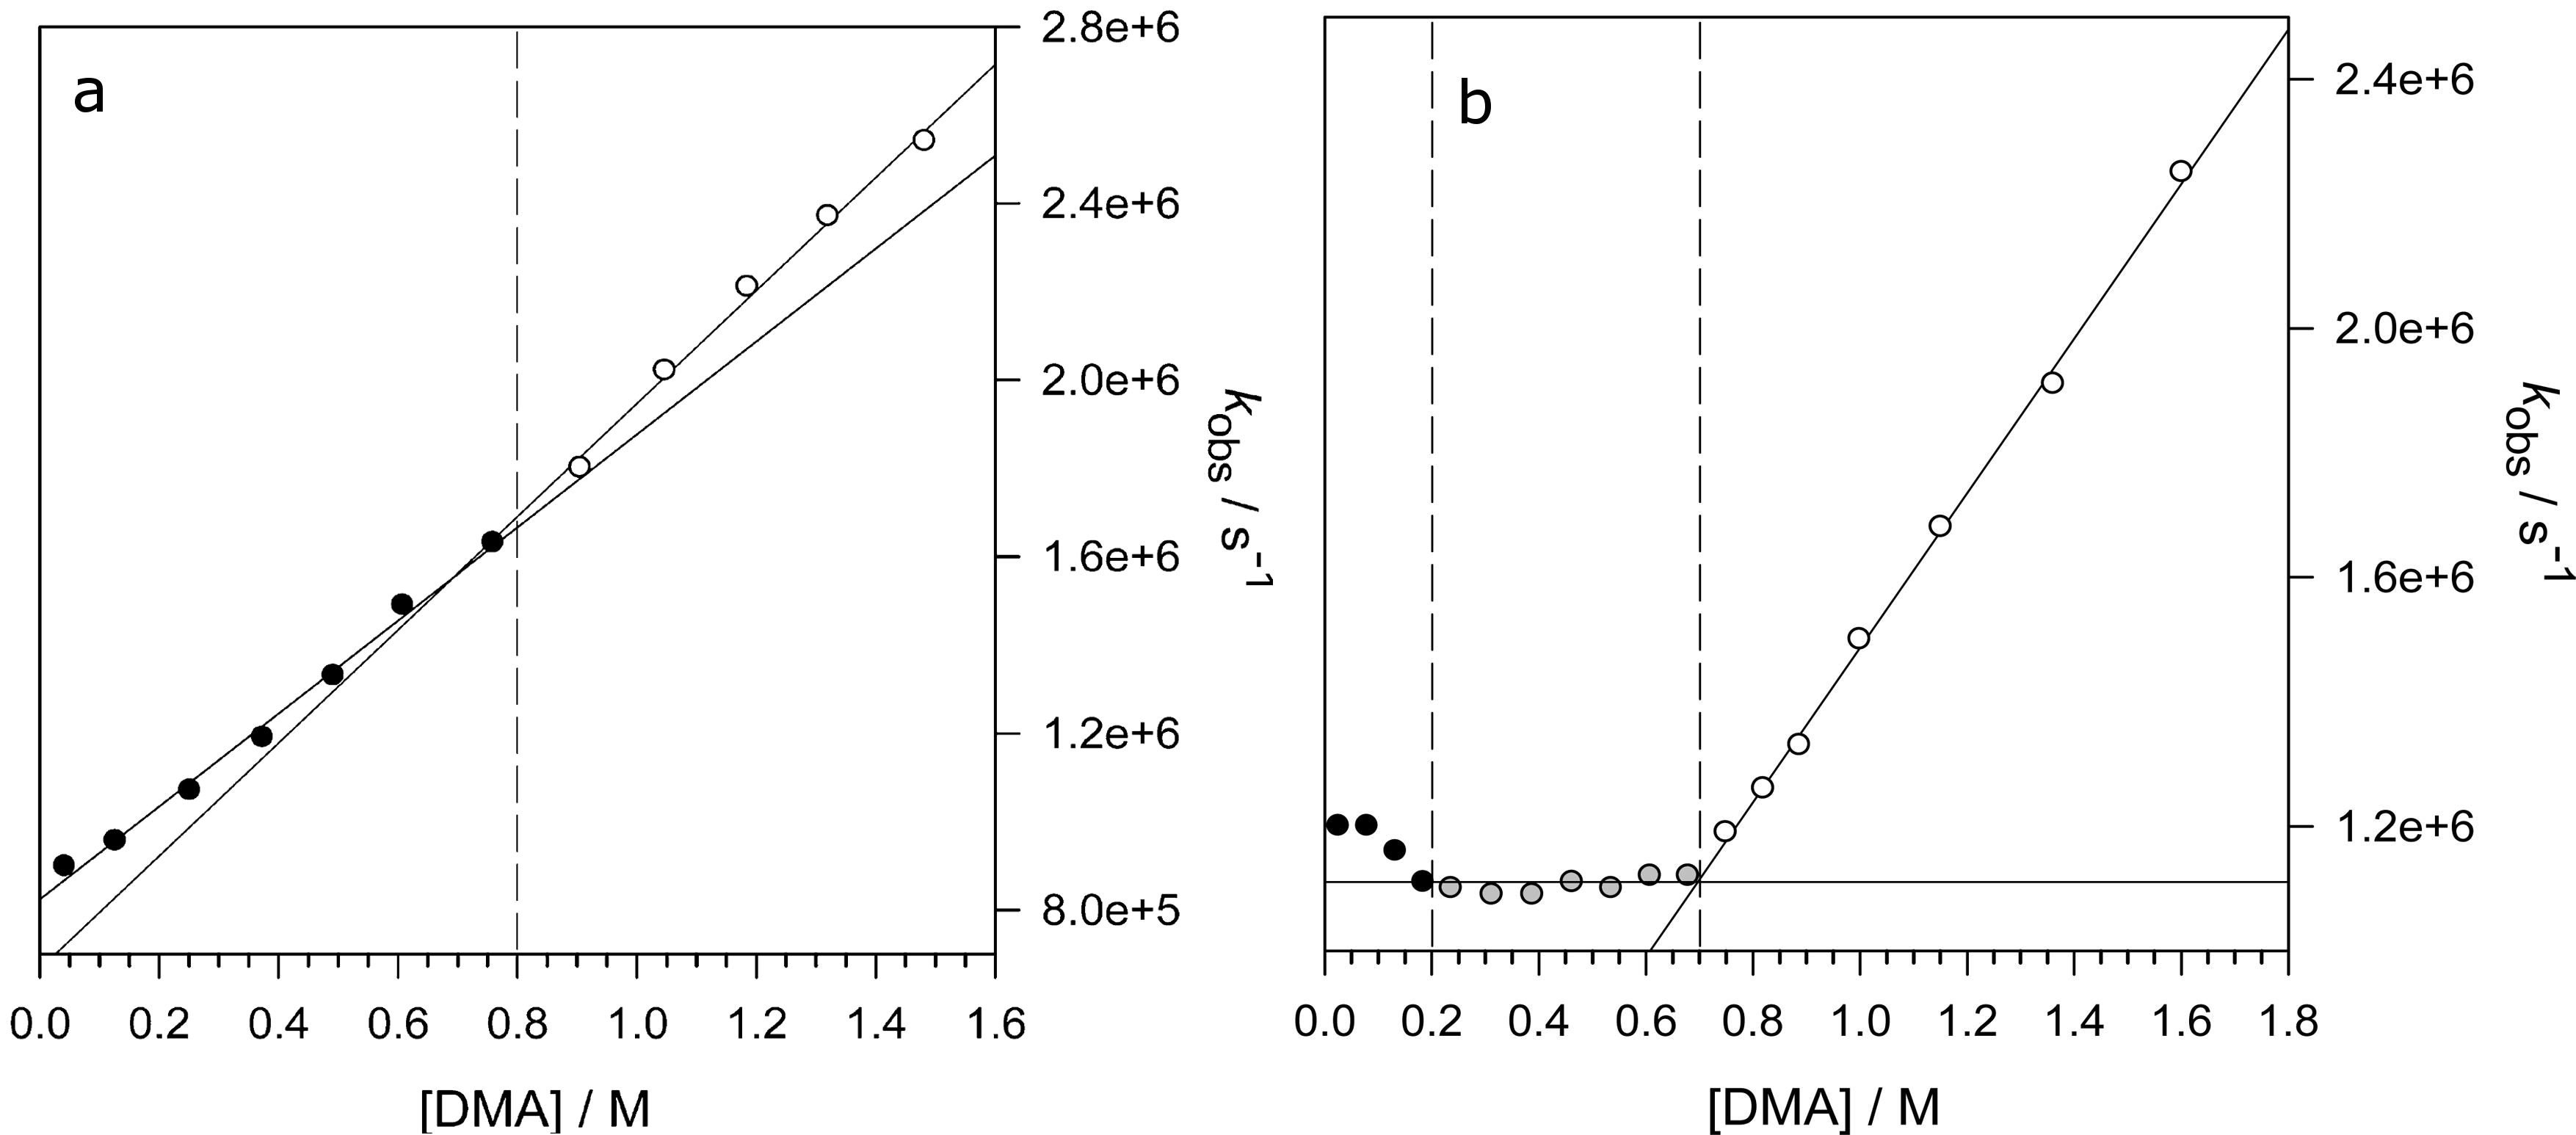
\includegraphics[width=\textwidth]{figures/exptdma-na-ca.png}
  \caption[Plot of observed rate constant against concentration of DMA for
  reaction with \cumo\ at 298 K in the presence of 0.2 M \ch{NaClO4} and
  \ch{Mg(ClO4)2}.] {\textbf{a)} Plot of observed rate constant against
	  concentration of DMA for reaction with \cumo\ at 298 K in the
	  presence of 0.2 M \ch{NaClO4}. 0--0.8 M [DMA] range (black circles),
	  $k_{H1}$ = 9.6\E{5} \Ms; 0.8--1.4 M [DMA] range (white circles),
	  $k_{H2}$ = 1.4\E{6} \Ms.  \textbf{b)} Plot of observed rate constant
  against concentration of DMA for reaction with \cumo\ at 298 K in the
  presence of 0.2 M \ch{Ca(ClO4)2}. 0.8--1.7 M [DMA] range (white circles),
  $k_{H1}$ = 1.2\E{6} \Ms. Adapted with permission from
  Reference~\protect\citenum{Salamone2015metals}. Copyright 2015 American
  Chemical Society.} \label{fig:k-metals-naca}
\end{figure}

Finally, \citet{Salamone2016} examined the effects of substrate structure on HAT
reaction between \cumo\ and sterically bulky tertiary alkanamides in the
presence of alkali and alkaline earth metal ions. For $N,N$-dialkylacetamides,
the steric bulk of the $N$-alkyl groups was previously
characterized.\cite{Salamone2014} Steric repulsion between \cumo\ and the
$N$-alkyl groups can decreases the HAT rate constant, as evident by the 3-fold
decrease in $k_H$ in going from DMA to $N,N$-diisobutylacetamide (DIA; 1.2\E{6}
and 3.1\E{5} \Ms, respectively). For reactions of \cumo\ with DIA addition of
0.2 M \ch{LiClO4} or \ch{Ca(ClO4)2} to results in the same trends in \ch{C-H}
bond deactivation observed for DMA. This indicates that the influence of metal
cation-substrate binding is not significantly influenced by the steric bulk of
$N$-alkyl groups.  The same is true for the addition of 0.2 M \ch{Mg(ClO4)2} to
abstraction from DIA by \cumo, as shown in~\ref{fig:k-dia-mg}. Once again, a
slight decrease in reactivity is observed for the first 2 equivalents of DIA,
followed by strong \ch{C-H} bond deactivation for an additional two equivalents,
and no deactivation beyond that. No additional insight was provided by Salamone
et al. as to the reason for this reactivity. The plausible explanation provided
was once again that \ch{Mg^{2+}} has a high charge density. These results show
that Lewis acid-base interactions between alkali or alkaline earth metal cations
can greatly depress hydrogen abstraction by alkyoxyl radicals.

\begin{figure}[!htbp]
  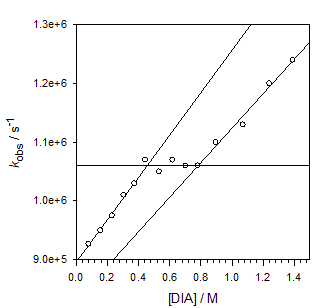
\includegraphics[width=0.6\textwidth]{figures/exptdia-mg.png}
  \caption[Plot of observed rate constant against concentration of DIA for
  reaction with \cumo\ at 298 K in the presence of 0.2 M \ch{Mg(ClO4)2}.]{Plot
	  of observed rate constant against concentration of DIA for reaction
	  with \cumo\ at 298 K in the presence of 0.2 M \ch{Mg(ClO4)2}. 0--0.4
	  M [DIA] range, $k_{H1}$ = 3.6\E{5} \Ms; 0.8--1.4 M [DIA] range,
	  $k_{H2}$ = 2.9\E{5} \Ms.  Reprinted from Tetrahedron, 72, Salamone et
  al., Hydrogen atom transfer from tertiary alkanamides to the cumyloxyl
  radical. The role of substrate structure on alkali and alkaline earth metal
  ion induced \ch{C–H} bond deactivation, 7757--7763, 2016, with permission
  from Elsevier.} \label{fig:k-dia-mg}
\end{figure}

With these results in mind, I am interested in the possibility that alkali and
alkaline earth metal cations found in biological system can protect \ch{C-H}
bonds in proteins from HAT to reactive oxygen-centred radicals. However, the
experimental results do not answer some of the key physico-chemical determinants
that may make this possible. Specifically, I have composed several important
research questions that remain unclear from the experimental results.

The first question I have is one of methodology: Can DFT-based methods can
accurately treat alkali/alkaline metal cation binding to organic substrates or
radicals? There exists limited ab initio data describing these
interactions.\cite{ Siu2001, Corral2003, Suarez2011, Baldauf2013} Therefore, I
have conducted a benchmark quality study involving \ch{Li^+}, \ch{Na^+},
\ch{Mg^{2+}}, \ch{K^+}, and \ch{Ca^{2+}}. To the best of my knowledge, this
represents the first systematic benchmark study of these metal cations with both
organic substrates and radicals.

Secondly, the nature of the binding of metal ions to substrates is still poorly
described, especially given the odd stoichiometric effects observed for
\ch{Mg(ClO4)2} with alkylamides. Specifically, I wish to address the range of
these interactions, and how much the metals effect the \ch{C-H} being broken. To
address this I have utilized both \ch{Na^+} and \ch{Mg^{2+}} in my calculations.
These metal ions were chosen to capture the large differences in Lewis acidity
and ion size associated with these third-period ions, and because they are two
of the most biologically relevant metal ions.

Thirdly, I address the effect that metal ions have on the HAT barrier heights.
Experiments demonstrate that under certain conditions, the presence of metal
ions can decrease HAT reactivity. If metal ions do effectively increase \ch{C-H}
bond strengths, this will be a contributing factor to the free energy barrier as
per the BEP principle\cite{Bell1936,Evans1938} (see Chapter~\ref{ch:bde}). There
will likely be additional factors such as polarization in the TS complex, or
other effects of possible charge transfer from the substrate to metal ions (or
vice versa). To investigate this, I have primarily studied HAT reactions
involving DMA and oxygen-centred radicals. Given there are only experimental
data for \cumo, this is the primary subject, however I was interested in
structural differences of the oxygen-centred radical, thus I have utilized \bno\
as well, which differs significantly in that it has the ability to form strong
pre-reaction complexes with hydrogen bond accepting
substrates.\cite{Salamone2012, Salamone2013} I also investigated the effect
metal cations have on the abstraction from DMA by the more biologically relevant
hydroxyl radical (See Appendix~\ref{ap:hat}). I have also performed calculations
with the bulkier DIA substrate and \cumo\ to verify whether or not steric bulk
does have an influence on the ability of a metal cation to affect HAT reactions.

Finally, given that reactions of DMA with \cumo\ in the presence of metal salts
show no deactivation, I was interested in studying the reactivity of alkoxyl
radicals with strong Lewis bases. Strong Lewis basic compounds are important as
they are often used as solvents in physical organic chemical experiments.
Furthermore, strong Lewis acids are common in biological systems. Specifically,
phosphates represent an important functionality as part of the DNA backbone, as
well being important in adenosine triphosphate (ATP), the so-called ``energy
currency.'' Sulphur containing amino acids are also susceptible to oxidation
into sulfoxides and disulfoxides.\cite{Lee2009} Therefore,
understanding the HAT reactivity of strong Lewis basic compounds with
oxygen-centred radicals also contributes to the understanding of oxidative
stress in biological systems.

HAT reactions involving alkoxyl radicals and strong Lewis bases have been
previously studied,\cite{Salamone2012, vanSanten2016} and can possess
interesting and unusual chemical reactivity. For instance, we recently showed
that for the HAT reaction between \bno\ and DMSO, \bno\ acts as a hydrogen atom
donor rather the acceptor.\cite{vanSanten2016} In light of this, I examined the
effect of metal cations on the expected HAT reactivity between \cumo\ and DMSO,
as well as the radical H-atom donation reactivity between \bno\ and DMSO. I also
performed calculations to determine the effects of metal cations and if there
exists reverse reactivity for two other strong Lewis basic substrates:
hexamethylphosphoramide (HMPA) and tributylphosphine oxide (TBPO). These results
are reported in Appendix~\ref{ap:hat}. The chemical structures of all the
species studies herein are shown~\ref{fig:hat-subs}.

\begin{scheme}[!htbp]
  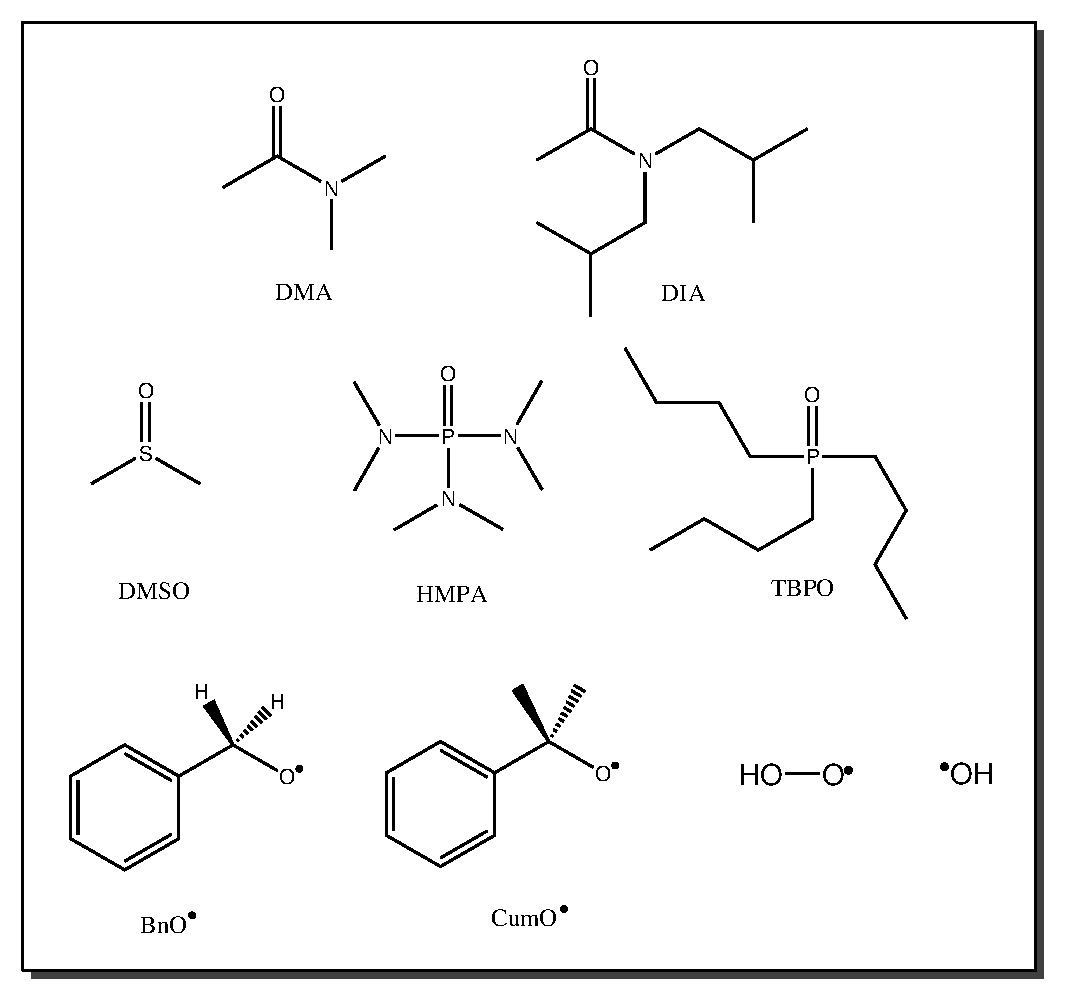
\includegraphics[width=\textwidth]{figures/Substrates.eps}
  \caption{Chemical structures of the species studied herein.}
  \label{fig:hat-subs}
\end{scheme}


\section{Computational methods and details}

All quantum mechanical calculations were performed using either the Gaussian 09
software package,\cite{Frisch2009} or the TURBOMOLE software
package.\cite{turbomole} Detailed benchmark studies of metal cation-substrate
interactions were carried out, the full data and discussion of which is
presented in Appendix~\ref{ap:hat}. Calculations for the benchmark quality data
of metal binding to substrates were first optimized at the
LC-$\omega$PBE-D3(BJ)/6-31+G(2d,2p) level of theory,\cite{Vydrov2006,
Vydrov2006a, Grimme2010, Johnson2006} and later re-optimized with larger
6-311+G(3df,3pd) basis sets. Single-point energy calculations were then carried
out using the coupled cluster methodology with single, double and perturbative
triples with full core correlation, CCSD(T,Full), and various basis sets. Final
benchmark quality binding energies have been calculated using the F12$^*$
explicitly correlated method with Def2-QZVPPD primary basis sets and Def2-QZVPP
auxiliary basis sets required for the resolution-of-the-identity (RI)
approximation as implemented in TURBOMOLE. The RI approximation is used to
reduce the computational cost associated with calculating MO
integrals.\bibnote{For a detail description of the RI approximation and explicit
correlation, see Ref.~\protect\citenum{OterodelaRoza2017}, Chapter 4.} A total
of 31 different DFT-based methods with nearly complete 6-311+G(3df,3pd) and
moderate sized 6-31+G(2d,2p) basis sets were tested both by single-point energy
calculations on the LC-$\omega$PBE-D3(BJ)/6-311+G(3df,3pd) optimized reference
structures. Geometry optimization calculations starting from the reference
structures were also performed for three of the best performing DFT-based
method, in order to verify their ability to capture the minimum energy bound
structures. The final DFT-based method selected from this benchmark work is
M05-2X.\cite{Zhao2006}

To test the effects of metal cations on HAT barrier heights, calculations were
first performed for the reactions not involving metal cations. Geometry
optimizations were performed at the M05-2X/6-31+G$^{**}$ level of
theory. Transition state (TS) structures were obtained by first freezing the
abstraction donor-hydrogen-acceptor bond lengths with multiple initial
orientations. The frozen bonds were then relaxed to obtain the final TS
structures, which were then used to identify the appropriate pre- and
post-reaction complexes. All structures were subjected to harmonic vibrational
frequency calculations, which were visualized using the Chemcraft
program\cite{ccraft} to verify minima (or saddle-points with a single imaginary
frequency connecting reactants to products for TS structures). Single-point
energy calculations were performed at the M05-2X/6-311+G(2d,2p) level of theory.
The effects of MeCN solvent were estimated by inclusion of the
SMD\cite{Marenich2009} continuum solvent model in single-point energy
calculations.

The inclusion of metal cations into the TS structures proved to be technically
challenging. It was my expectation that I could simply include metal cations and
necessary counter-anions into the minimum energy complex structures and
re-optimize, however this was not the case. TS structures were once again
obtained by constrained optimization with the inclusion of the metal cation and
counter-anion and freezing the abstraction donor-hydrogen-acceptor bond lengths,
providing a guess TS structure. However, in most cases the force constants
(which are necessary for a TS optimization calculation) from the guess TS
structure were not representative of the true TS structure, thus force constants
were recalculated for every step along the optimization, using the ``CalcAll''
keyword in Gaussian. This is a very computationally expensive procedure. Even
using this method, many TS structures including metal cations failed to
converge. Therefore, guess TS structures that contain a single imaginary
frequency connecting reactants to products are used in place. This technique
provides genuine TS structures, although they may not be the TS associated with
the minimum energy reaction pathway. Nonetheless, the guess TS structure can be
used to provide an estimate of the reaction barrier height that are verified
with calculations that were successful. Where available, final TS structures
were used to identify the appropriate pre- and post-reaction complexes.

Natural bond order (NBO) and natural population analysis (NPA) were utilized in
order to investigate the electronic structures involved in the HAT reactions and
the effects of metal cation binding.\cite{Reed1983, Reed1985, Glendening2012}
Version 3.1 of the NBO software package,\cite{NBO3} as implemented in the
Gaussian 09 package was used in all cases.\cite{Frisch2009} NBO analysis
provides a means for estimating the physical effects of chemically intuitive
orbital interactions while NPA charges are a means for calculating the
occupancies and charges of atomic centres.\cite{Landis2014, Weinhold2016}

\section{Exploring the nature of metal cation substrate interactions}

The first step to understanding the effect non-redox active metal have on HAT
reaction barrier heights is investigating the nature of the binding interaction.
\ref{fig:pes-dma-na}a,b show the potential energy surfaces (PESs) of the binding
of sodium ion, and sodium chloride to DMA, respectively. There are three
surfaces in each plot representing the same potential energy surface in the
gas-phase (black circles), and in an SMD\cite{Marenich2009} continuum solvent
field of MeCN (grey squares) or water (white circles). For both sodium ion and
sodium chloride, the gas-phase PES demonstrates strong binding with respect to a
solvated system. This is indicated by a much deeper well than both solvents and
a long-range interaction that does not tail off within 6 \AA\ due to the lack of
screening. This underscores the importance of including solvent effects in
studying the effects of metal cations. Interestingly, for the effects of water
compared to MeCN solvent appears to be quite small. In both cases the difference
between the minimum of the water PES is about 2.5 \kcalmol. Furthermore, the
minimum of the PES well in all cases falls at about the same distance (2.1--2.2
\AA) in the gas-phase and in both solvents. The small differences in binding
interactions indicate that the effects as measured in MeCN may also apply to the
more biologically relevant aqueous system.

For both the ion and the salt of sodium in water and MeCN, the binding
interaction only approaches zero slowly. Even at 6 \AA, the predicted binding
energy of DMA in water with \ch{Na^+} and \ch{NaCl} are 1.1 and 0.7 \kcalmol,
respectively. This is an indication that M05-2X-SMD does not properly capture
long-range interactions of DMA with sodium. This may be a result of not fully
capturing the screening effect of solvent. Nonetheless, at a distance of 5 \AA,
which corresponds well with the size of the first solvation shell of the sodium
ion,\cite{Degreve1996} the interaction between DMA and sodium is nearly zero.
This result is consistent with literature that studies the Hofmeister series,
where it has been shown that biologically relevant cations are only able to
influence their immediate solvation shell.\cite{Omta2003, Funkner2011}
Furthermore, \citet{Heyda2009} utilized molecular dynamics simulations of
$N$-methylacetamide in aqueous solutions of NaCl, NaBr, KCl, and KBr to obtained
radial distribution functions (RDFs). The RDFs are in agreement with the
calculated PESs in that the most probable distance to find \ch{Na^+} from the
amidic oxygen-centre is at about 2--2.5 \AA\ separation. Heyda et al. also
showed that \ch{Na^+} binds more strongly with the amide than \ch{K^+}, and that
the nature of the halide counteranion does not contribute significantly to the
overall interaction. This is consistent with the results of Salamone et al.,
which showed that the nature of the counteranion plays a negligible role to the
effect on rate constants.\cite{Salamone2013a} The calculated binding energies of
\ch{NaCl} and \ch{NaClO4} to DMA are very similar in magnitude (-16.0 and -18.1
\kcalmol, respectively). From these results it is possible to draw an important
conclusion: The use of \ch{Cl^-} in the calculations may reasonably reflect the
trends observed by Salamone et al.  with \ch{ClO4^-} and \ch{OTf^-}.

\begin{figure}[!htbp]
\centering
\vspace{1.0cm}
\hspace*{-1.2cm}
\begin{minipage}{8cm}
  \centering
  \begin{overpic}[width=\textwidth]{figures/pes_dma_na}
  \put(5,70) {\large\textbf{a.}}
\end{overpic}
\end{minipage}%
\begin{minipage}{8cm}
  \centering
  \begin{overpic}[width=\textwidth]{figures/pes_dma_nacl}
  \put(5,70) {\large\textbf{b.}}
\end{overpic}
\end{minipage}
\caption[Potential energy surface of binding energy between DMA and sodium
cation and sodium chloride.]{Potential energy surface of binding energy between
DMA and \textbf{a)} sodium cation and \textbf{b)} sodium chloride as a function
of O-Na interaction distance (\AA). The black line and points represent
gas-phase results, the grey squares and line is in continuum MeCN solvent, and
white circles and dashed line is in continuum water solvent. Calculated as a
rigid scan from the M05-2X/6-31+G$^{**}$ minimized complex structure at the
M05-2X/6-311+G(2d,2p) level of theory with the SMD solvent model.}
\label{fig:pes-dma-na}
\end{figure}

\ref{fig:pes-dma-mg}a,b show the PESs of the binding of magnesium ion, and
magnesium dichloride to DMA, respectively. As is the case for \ch{Na^+}, the
gas-phase PES of \ch{Mg^{2+}} is very strongly bound. In fact, the binding
energy does not asymptotically approach zero. At an O--Mg distance of 12 \AA,
there is calculated binding interaction of -48.5 \kcalmol, which is actually
greater than at 6 \AA\ by about 5 \kcalmol. This is a result of the the
ionization potentials (IP) of the metals with respect to that of DMA. The
experimental IP\cite{Slifkin1967, Baldwin1977, CRC2016} of DMA is 8.8--9.2 eV,
the first IP of Na is 5.1 eV, and the second IP of Mg is 15.0 eV (calculated
with M05-2X/6-311+G(2d,2p) = 8.9, 5.0, and 14.9 eV, respectively). In a solvated
system, magnesium ions exist invariably in the +2 oxidation state, however, due
to nature of the IPs, DFT-based methods prefer to transfer charge, resulting in
a non-convergent binding interaction between DMA and \ch{Mg^2+}, but not for
\ch{Na+}.

\begin{figure}[!htbp]
\centering
\vspace{1.0cm}
\hspace*{-1.2cm}
\begin{minipage}{8cm}
  \centering
  \begin{overpic}[width=\textwidth]{figures/pes_dma_mg}
  \put(5,70) {\large\textbf{a.}}
\end{overpic}
\end{minipage}%
\begin{minipage}{8cm}
  \centering
  \begin{overpic}[width=\textwidth]{figures/pes_dma_mgcl2}
  \put(5,70) {\large\textbf{b.}}
\end{overpic}
\end{minipage}
\caption[Potential energy surface of binding energy between DMA and magnesium
cation and magnesium chloride.]{Potential energy surface of binding energy
between DMA and \textbf{a)} magnesium cation and \textbf{b)} magnesium chloride
as a function of O-Mg interaction distance (\AA). The black line and points
represent gas-phase results, the grey squares and line is in continuum MeCN
solvent, and white circles and dashed line is in continuum water solvent.
Calculated as a rigid scan from the M05-2X/6-31+G$^{**}$ minimized complex
structure at the M05-2X/6-311+G(2d,2p) level of theory with the SMD solvent
model.} \label{fig:pes-dma-mg}
\end{figure}

The inclusion of MeCN and water solvent appear at first glance to alleviate this
problem. Note however that both PESs cross over zero binding at about 3 \AA,
indicating there is still charge transfer to some extent. Additionally, for
magnesium chloride in the gas-phase, there also appears to be charge transfer
occurring, as evident by the PES crossing zero just below 4 \AA. On the other
hand, the inclusion of either water or MeCN solvent with \ch{MgCl2} give
reasonable PESs with a binding interaction of about -25 \kcalmol\ for both water
and MeCN, and a tailing off at about 3 \AA, or slightly larger than the size of
the first hydration shell of \ch{Mg^2+} (ca. 2 \AA).\cite{Chatterjee2013}
Therefore, studying the effects of magnesium on HAT reaction barrier may be
possible using \ch{MgCl2}, however given the difficulties with Mg in general, I
elected to focus only on \ch{NaCl} for future considerations.

Next, I performed calculations to determine if the interaction of metal cations
systematically increase the bond strengths of \ch{C-H} bonds in the models of
interest in this work. This effect is hypothesized to occur due to a decrease in
electron density in the \ch{C-H} $\sigma^*$ orbital, which is normally present
due to hyperconjugative overlap. The BDEs for several substrates in the presence
of \ch{Na^+} and \ch{NaCl} are listed in~\ref{tab:bde-metal}. The ROCBS-QB3 BDEs
for each of the substrates is included to demonstrate that the relative order of
BDEs for substrates with multiple \ch{C-H} bonds is reasonable. The BDE for an
arbitrary metal substrate complex (\ch{M\bond{dotted}X-H}) can be calculated as:

\begin{equation}
BDE = E(\ch{M\bond{dotted}X^.}) + E(\ch{H^.}) - E(\ch{M\bond{dotted}X-H})
\end{equation}

\begin{table}[!htbp]
  \caption[Bond dissociation enthalpies of DMA, DMSO, MeCN, and DIA with and
  without metal cations.]{Bond dissociation enthalpies of DMA, DMSO, MeCN, and
  DIA with \ch{Na^+}, \ch{NaCl}, and without metal cations (Bare) calculated at
  the M05-2X-SMD(MeCN)/6-311+G(2d,2p)//M05-2X/6-31+G$^{**}$ level of theory.
  ROCBS-QB3-SMD(MeCN) BDEs without metals are included for reference. All values
  are in \kcalmol.} \label{tab:bde-metal}
  \begin{tabular}{l c c c c}
                    & ROCBS-QB3 & \multicolumn{3}{c}{M05-2X} \\
                    \cline{2-5}
    Substrate       & Bare      &    Bare    &\ch{Na+}    &\ch{NaCl}   \\
    \hline
    DMA (acetyl)    & 101.0 & 98.5 & 97.8 & 98.4 \\
    DMA (cis)       & 94.8 & 92.2 & 93.2 & 94.0 \\
    DMA (trans)     & 94.3 & 91.6 & 92.8 & 92.6 \\
    DMSO            & 104.3 & 103.4 & 104.4 & 103.7 \\
    MeCN            & 99.0 & 97.4 & 98.3 & 98.1 \\
    DIA (acetyl)    & 99.7 & 97.8 & 97.5 & 97.7 \\
    DIA ($\alpha$-cis)  & 97.0 & 95.7 & 96.5 & 95.3 \\
    DIA ($\beta$-cis)   & 98.3 & 96.4 & 94.8 & 93.1 \\
    DIA ($\alpha$-trans)& 94.6 & 93.0 & 93.8 & 94.0 \\
    DIA ($\beta$-trans) & 97.3 & 95.3 & 95.5 & 95.5
  \end{tabular}
\end{table}

For DMA, the $N$-methyl groups cis and trans relative to the carbonyl are the
weakest, and therefore most thermodynamically favourable for abstraction.
\citet{Salamone2013} showed that both \bno\ and \cumo\ prefer to abstract from
the $N$-methyl groups of DMA, rather than the acetyl group. The complexation of
\ch{Na^+} increases the cis BDE by 1.0 \kcalmol\ and the trans BDE by 1.2
\kcalmol. The complexation of \ch{NaCl} to DMA increases the cis BDE by 1.8
\kcalmol\ and the trans BDE by 1.0 \kcalmol. One would expect the greater
positive charge of the sodium cation (as compared to the sodium moiety of
\ch{NaCl}) to have a greater effect on the BDEs, however these calculations
indicate this may not always be the case. Specifically, the cis BDE is 0.8
\kcalmol\ weaker for the \ch{DMA-NaCl} complex as compared to the \ch{DMA-Na^+}
complex. These results, which are inconsistent with the hypothesis, can be
explained by additional analysis of both the parent and radical complexes. The
structures of the DMA-NaCl complex and three possible radical complexes are
shown in~\ref{fig:dma-na-cl}a-d.

\begin{figure}[!htbp]
	\centering

	\subfigure[DMA-NaCl]{
		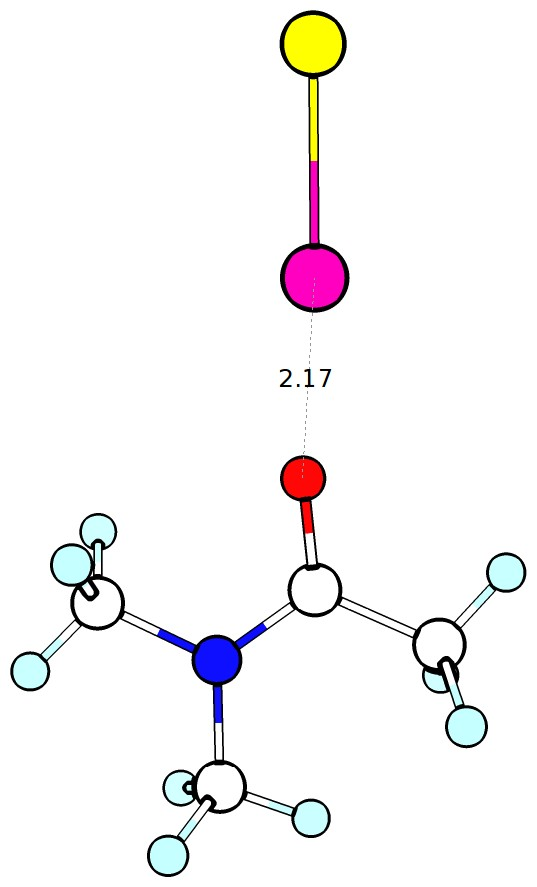
\includegraphics[width=4cm]{figures/dma-na-cl}
	}
  \subfigure[Acetyl radical]{
		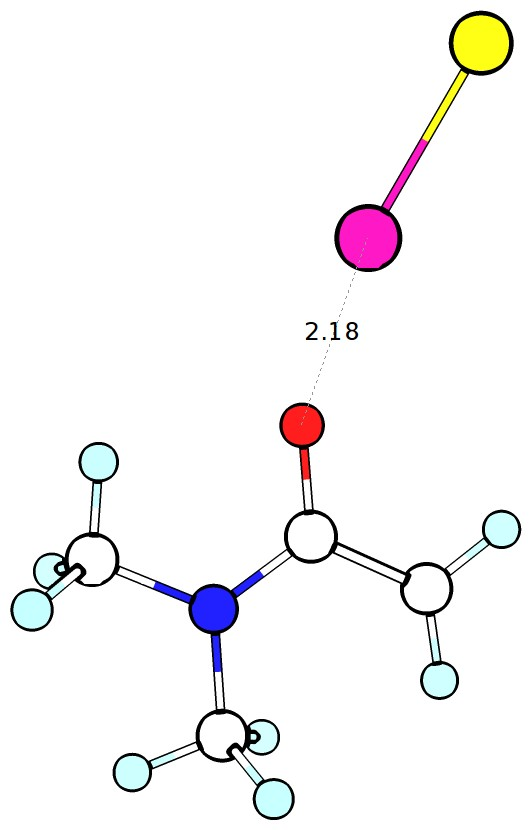
\includegraphics[width=4cm]{figures/dma-na-cl-acetyl}
	}
  \subfigure[Cis radical]{
    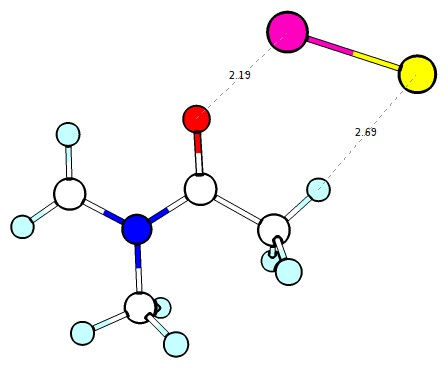
\includegraphics[width=6cm]{figures/dma-na-cl-cis}
  }
  \subfigure[Trans radical]{
    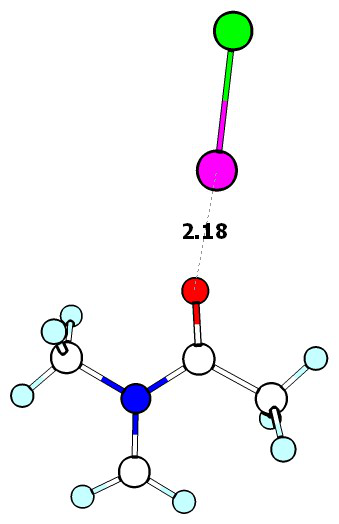
\includegraphics[width=4cm]{figures/dma-na-cl-trans}
  }

\caption[Structures of the DMA-NaCl complex and associated radical
complexes.]{Structures of \textbf{a} the DMA-NaCl complex, \textbf{b} the
DMA-NaCl acetyl radical complex, \textbf{c} the DMA-NaCl cis
radical complex, and \textbf{d} the DMA-NaCl trans radical complex. Key
interaction distances are shown in units of \AA. Element colour key: white is
carbon, light blue is hydrogen, red is oxygen, blue is nitrogen, purple is
sodium, and green is chlorine.} \label{fig:dma-na-cl}
\end{figure}

NBO analysis can be used that give a qualitative description based on
perturbation theory of the energy contribution of specific NBO orbital
interactions.\cite{Weinhold2016} Using NBO analysis on DMA, the estimated effect
of hyperconjugative overlap reveals a weakening of the $N$-methyl \ch{C-H} bonds
by approximately 5.6 and 5.9 \kcalmol\ for the cis and trans positions,
respectively. Upon complexation of \ch{Na^+}, the bond weakening effects become
3.7 and 4.1 \kcalmol\ for the cis and trans positions, respectively. Therefore,
from an NBO perspective, the cis an trans $N$-methyl bond strengths can be
described as strengthening upon complexation of \ch{Na^+}. Furthermore, the
predicted effect of hyperconjugative overlap in the \ch{DMA-NaCl} complex are
5.4 and 5.5 \kcalmol\ for the cis and trans positions, respectively. Again, from
an NBO perspective, the complexation of \ch{NaCl} can be said to strengthen the
$N$-methyl \ch{C-H} bonds in DMA, but not as much as \ch{Na^+}. NBO analysis of
the parent complexes thus supports the hypothesis.

However, BDEs can be affected by both parent and radical stability. The
hypothesis considers only the stability of the parent molecule, where
complexation of a metal cation stabilizes the parent by withdrawing electron
density from an anti-bonding orbital. In the case of complexation of \ch{NaCl},
secondary interactions between the Cl moiety of \ch{NaCl} and the radical can
result in the destabilization of the radical complex and a further increase in
the predicted \ch{C-H} BDE. This is the case for the cis-DMA-NaCl radical
complex (\ref{fig:dma-na-cl}c). The Cl moiety of \ch{NaCl} is attracted to the
partial positive charge of the acetyl hydrogen of DMA, which is greater than the
partial charge on the cis $N$-methyl hydrogens (0.25 $e^-$ vs. 0.21 $e^-$). This
leads to the donation of electron density from Cl to the \ch{C-H} $\sigma^*$
orbital. NBO estimates this orbital interaction to amount to about 1 \kcalmol\
of bond weakening. Therefore, the hypothesis is incomplete in that it does not
account for radical complex stability. Furthermore, with respect to TS
complexes, additional interactions may further complicate the picture.

Interestingly, the predicted BDE for the acetyl position of DMA decreases,
rather than increasing as hypothesized, with both \ch{Na^+} and \ch{NaCl}. This
can be attributed to the change in electronic structure associated with the
complex. Consider the two possible resonance forms of DMA shown in
~\ref{fig:dma-res}. Glendening and Hrabal\cite{Hrabal1997} utilized natural
resonance theory to estimate that the right-hand resonance structure in the
closely related formamide contributes about 30\% to the overall resonance
hybrid. On the other hand, NBO analysis predicts a bond order in DMA of 1.5
between the C and O and the C and N. Nonetheless, the complexation of DMA to
\ch{Na^+} slightly increases the contribution of the zwitterionic form,
resulting in a decrease in electron density at the carbonyl carbon. This is
evidenced by the increase in NPA charge at the carbonyl carbon from +0.72 in DMA
to +0.74 in the DMA-\ch{Na^+} complex. The partially positively-charged carbon
centre inductively withdraws electron density, stabilizing the acetyl radical,
increasing the $\pi$-bonding character between the two carbon centres, and
decreasing the effective BDE.

The observed inductive effects also manifests in the decrease in the
carbonyl-acetyl C-C bond lengths in the acetyl radical, which decrease from
1.457 \AA\ to 1.443 \AA\ upon complexation of \ch{Na^+}. Complexation of
\ch{NaCl} results in a bond length of 1.451 \AA. These results are consistent
with the ordering of the calculated acetyl BDEs (DMA \textgreater\ \ch{DMA-NaCl}
\textgreater\ \ch{DMA-Na^+}). On the other hand, the amidic nitrogen becomes net
more positive upon complexation of either \ch{Na^+} or \ch{NaCl}, but still has
an NPA charge that is negative. As a results, there is no inductive
stabilization effect for the $N$-methyl radical complexes.

\begin{figure}[!htpb]
  \centering
  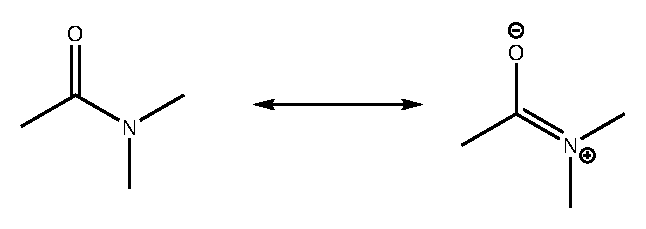
\includegraphics[width=0.7\textwidth]{figures/DMA-resonance.eps}
  \caption{The resonance forms of DMA.}
  \label{fig:dma-res}
\end{figure}

For MeCN and DMSO the complexation of either \ch{Na^+} or \ch{NaCl} results in
an increase in \ch{C-H} BDE.\@ In MeCN, the electron density in the \ch{C-H}
$\sigma^*$ anti-bonding orbital decreases as a result of the interaction between
\ch{Na} and the nitrogen centre. DMSO has a non-Lewis electronic structure,
making it difficult to analyze orbital interactions of valence-bond orbitals.
Nonetheless, there is normally hyperconjugative overlap between the sulphur
centre and the \ch{C-H} $\sigma^*$ anti-bonding orbitals, which was confirmed by
NBO analysis. The electron density in the \ch{C-H} $\sigma^*$ orbital decreases
as a result of the interaction of \ch{Na^+} with the oxygen-centre of DMSO.

Upon complexation of \ch{NaCl}, the BDEs of the more sterically bulky amide
substrate DIA follow the same trend that is observed as for DMA: The acetyl
\ch{C-H} BDE decreases due to inductive stabilization, while the \ch{C-H} bonds
$\alpha$ to the amidic nitrogen centre increase as a result of decreased
\ch{C-H} $\sigma^*$ occupancy. Alkoxyl radicals are not expected to abstract
from \ch{C-H} BDEs of the bonds $\beta$ to the nitrogen centre in DIA or other
longer chain $N$-alkyl amides, as the incipient radical is not stabilized by the
amidic $\pi$-system. However, due to steric repulsion, the $\alpha$-radicals of
DIA cannot lie directly plane of allowing conjugation with the $\pi$-system. As
such the $\alpha$-\ch{C-H} BDEs of DIA are greater than those of DMA by 2-3
\kcalmol, and are closer to the $\beta$-\ch{C-H} BDEs than perhaps expected. The
effects of sodium binding to the amidic oxygen are almost nil for the
$\beta$-trans \ch{C-H} bond of DIA, however there is a significant decrease in
the $\beta$-cis \ch{C-H} BDE. \ref{fig:dia-na-cl}a,b shows the structures of the
DIA-NaCl complex and the $\beta$-cis radical complex, where it can seen that the
metal cation interacts with both the oxygen-centre and the carbon-centred
radical. This interaction stabilizes the radical complex and thus decreases the
effective BDE, however this interaction is likely not possible in the TS
structure and is not expected to contribute to a reduction of the barrier
height.

\begin{figure}[!htbp]
	\centering

	\subfigure[DIA-NaCl]{
		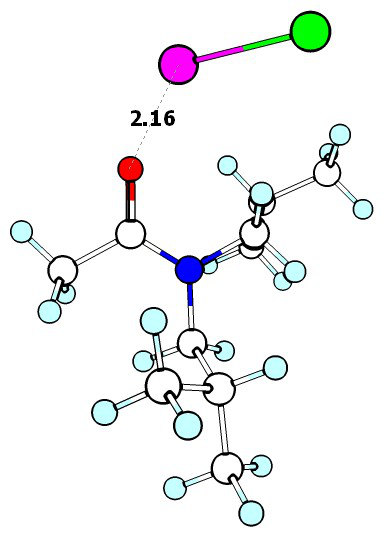
\includegraphics[width=5cm]{figures/dia-na-cl}
	}
  \subfigure[$\beta$-cis radical]{
		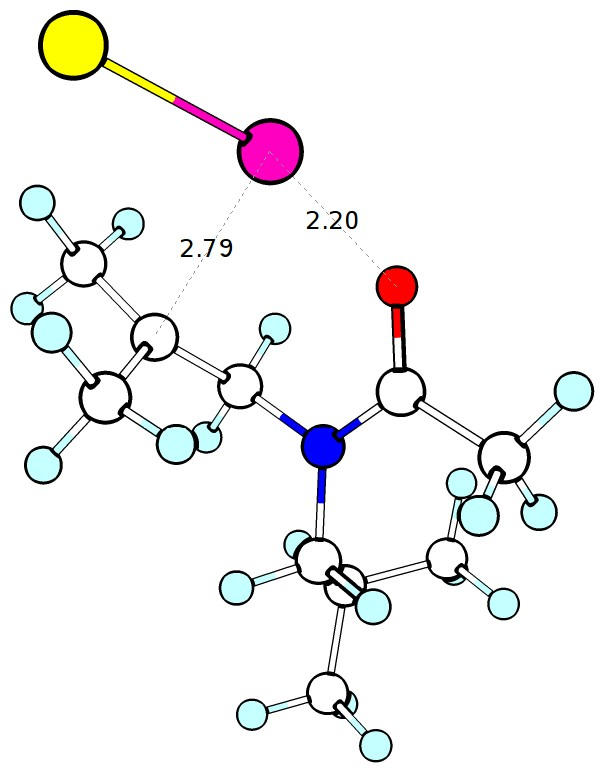
\includegraphics[width=5cm]{figures/dia-na-cl-rad-b}
	}

  \caption[Structures of the DIA-NaCl complex and radical complex.]{Structures
  of \textbf{a} the DMA-NaCl complex, \textbf{b} the DIA-NaCl $\beta$-cis
  radical complex. Key interaction distances are shown in units of \AA. Element
  colour key: white is carbon, light blue is hydrogen, red is oxygen, blue is
  nitrogen, purple is sodium, and green is chlorine.} \label{fig:dia-na-cl}
\end{figure}

All of these results together confirm that specific metal-substrate interactions
can increase the effective BDEs of abstractable \ch{C-H} bonds by decreasing
\ch{C-H} $\sigma^*$ occupancy. However, this is complicated by the possibility
for secondary interactions between the metal or counter-anion with the formed
radicals. Furthermore, additional factors such as induction can alter the
effects. It appears that for \ch{C-H} bonds $\alpha$ to atoms with LPs that
hyperconjugatively overlap with the \ch{C-H} $\sigma^*$ anti-bonding orbital,
the complexation of non-redox active metals increases the \ch{C-H} bond
strength. However, if the \ch{C-H} bond is adjacent to an electron-poor centre,
such as the carbon of a carbonyl, metal complexation actually decreases the bond
strength slightly by stabilizing the carbon-centred radical. In the context of
HAT reaction barrier heights, increasing the effective \ch{C-H} bond strength
should decrease the reaction-rate slightly by destabilizing the TS complex.
However, there are other important factors to consider such as how the metal
effects the dipole moment in the TS complex. Furthermore, it is important to
note that experiments showed that \ch{NaClO4} did not significantly effect the
HAT rate constants for reactions between \cumo\ and organic substrates.
Therefore, the effects observed herein likely are an exaggeration of what is
truly occurring in situ. Nonetheless, these theoretical calculations may be
useful in developing an understanding of the subtle nature of the effects of
non-redox active metal cations on HAT reactions in general.

With regards to the implications these results have on protein systems, since
abstraction occurs predominantly from an $\alpha$-\ch{C-H} bonds, it is likely
that the nature of the amino acid, and the three dimensional structure of the
protein will have significant importance. As the geometry of the peptide
backbone becomes more strained by steric interactions, the $\alpha$ hydrogen
will become more difficult to abstract, as might be exemplified by the higher
\ch{C-H} BDEs in DIA as compared to DMA. In the absence of secondary
interactions, alkali or alkaline earth-metals are able to bind to a given
carbonyl site on the surface of a protein, they may exert a chemo-protective
effect by increasing the BDE of an adjacent \ch{C-H} bond. However, the
complexity of biological systems makes the absence of secondary interaction
unlikely. Therefore, the possibility for chemo-protection to occur is remote.

\section{HAT reactions involving non-redox active metals}

\subsection{DMA}

Hydrogen abstraction reactions involving the oxygen-centred radicals \bno\ and
\cumo\ and DMA in MeCN have been previously investigated experimentally and
theoretically.\cite{Salamone2013} The HAT reaction between DMA and \bno\ was
determined to occur predominantly through a direct HAT mechanism from the
$N$-methyl group cis relative to the carbonyl, and is kinetically limited by the
formation of a strong pre-reaction complex between the relatively acid
$\alpha$-C-H of \bno\ and the amidic oxygen centre. On the other hand, \cumo\
cannot form a strong hydrogen-bonding interaction, and thus forms a
non-specific dispersion-bound pre-reaction complexes. Abstraction by \cumo\
still takes place from one of the $N$-methyl groups, but the rate constant is 2
orders of magnitude less than for \bno. Recall that the inclusion of metal salts
in reactions of DMA with \cumo\ were previously
investigated.\cite{Salamone2015metals} On the basis of the exaggerated effects
observed in the changes in BDEs and the technical difficulties associated with
these studies, the goal of this work is not to reproduce experimental results,
but rather, develop insights into the possible changes that can occur as a
result of metal salt addition to HAT reactions.

Herein, I have calculated the reaction barrier heights for all three
abstractable positions of DMA for HAT reactions involving \cumo\ and \bno, both
with and without \ch{NaCl}. These data are summarized in~\ref{tab:DMA-dG}.
Perhaps alarmingly, the free energy barriers calculated at the
M05-2X-SMD(MeCN)/6-311+G(2d,2p)//M05-2X/6-31+G$^{**}$ are systematically higher
than those previously calculated by about 8.5 \kcalmol.\cite{Salamone2013} The
previously calculated results were in reasonable agreement with experimental
results. The reason for this discrepancy is unclear, given that M05-2X has
previously been used successfully to calculate accurate HAT rate
constants.\cite{Galano2013} Furthermore, the optimized minimum energy structures
from both methods do not differ significantly, with the exception of slightly
shorter abstracting \ch{C-H} partial bonds and slightly elongated \ch{O-H}
partial in the TS structures excluding \ch{NaCl} (ca. 0.03 to 0.05 \AA).
However, the relative ranking and differences in energies for the reaction
barrier heights for the different \ch{C-H} bonds are consistent with previous
results. Therefore, although these results cannot be used to predict rate
constants, they are useful for studying the change in barrier height due to the
addition of NaCl.

\begin{table}[!htbp]
\caption[Calculated free energy (enthalpy) barrier for direct HAT from different
\ch{C-H} bonds in DMA by \cumo\ and \bno, with and without
\ch{NaCl}.]{Calculated free energy (enthalpy) barrier ($\Delta G(H)^\ddagger$,
\kcalmol) for direct HAT from different \ch{C-H} bonds in DMA by \cumo\ and
\bno, with and without \ch{NaCl}. The change in barrier height ($\Delta \Delta
G(H)^\ddagger$) is calculated relative to the same abstraction site without the
inclusion of \ch{NaCl}. All barrier heights are relative to separated reactants
(or complexed DMA-NaCl) and were calculated at the
M05-2X-SMD(MeCN)/6-311+G(2d,2p)//M05-2X/6-31+G$^{**}$ level of theory.}
\label{tab:DMA-dG}
  \begin{tabular}{l l c c}
Reaction   & Abstraction Site &  $\Delta G(H)^\ddagger$ & $\Delta\Delta G(H)^\ddagger$ \\
\hline
DMA + \cumo   &  trans              &  17.3(3.4)           &              \\
              &  cis                &  17.5(3.8)           &              \\
              &  acetyl             &  21.6(7.5)           &              \\
DMA-NaCl + \cumo &  trans              &  20.3(3.7)        &    3.0(0.3)  \\
              &  cis                &  18.4(1.2)           &    0.9(-2.6) \\
              &  acetyl             &  21.0(4.3)           &   -0.6(-3.2) \\
DMA + \bno    &  trans              &  16.5(3.7)           &              \\
              &  cis                &  17.5(3.6)           &              \\
              &  acetyl             &  20.8(7.8)           &              \\
DMA-NaCl + \bno &  trans              &  18.6(1.7)         &    2.1(-2.0) \\
              &  cis                &  17.8(4.7)           &    0.3(1.1)  \\
              &  acetyl             &  22.0(4.7)           &    1.2(-3.1)
  \end{tabular}
\end{table}

Focussing first on the barrier heights for HAT between DMA and \cumo, the
results of complexation with \ch{NaCl} is variable. For each of the acetyl, cis,
and trans \ch{C-H} bond positions of DMA, there are three distinct effects upon
complexation of \ch{NaCl}. For the trans position, both the free energy and
enthalpic barriers increase, for the cis position the free energy barrier
increases and the enthalpic barrier decreases, and for the acetyl position both
the free energy and enthalpic barriers decrease. The reasons for this can be
understood by examining the TS structures, which are shown
in~\ref{fig:dma-cumo-ts}a-f.

\begin{figure}[!htbp]
  \setcounter{subfigure}{0}
  \centering

  \subfigure[Trans DMA + \cumo]{
		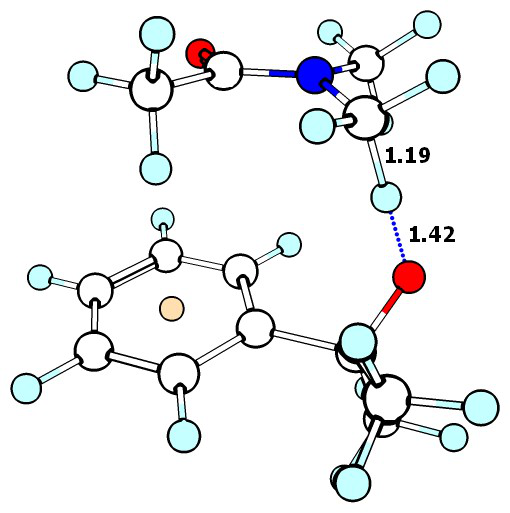
\includegraphics[width=5cm]{figures/dma-cumo-trans}
	}
  \subfigure[Trans DMA-NaCl + \cumo]{
		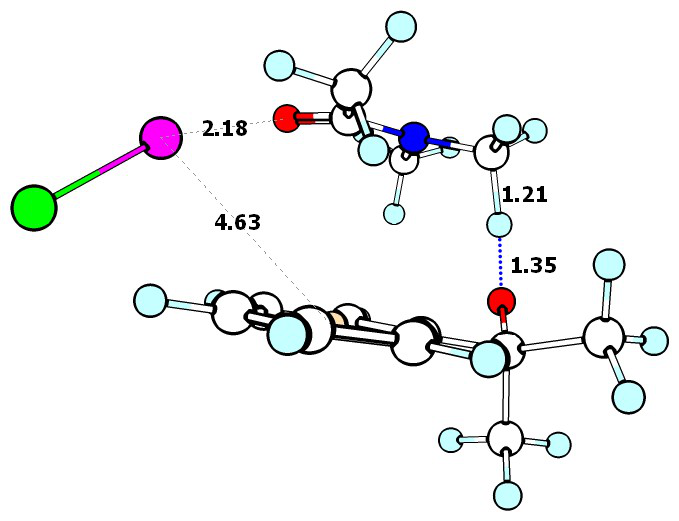
\includegraphics[width=5cm]{figures/dma-nacl-cumo-trans}
	}

  \subfigure[Cis DMA + \cumo]{
    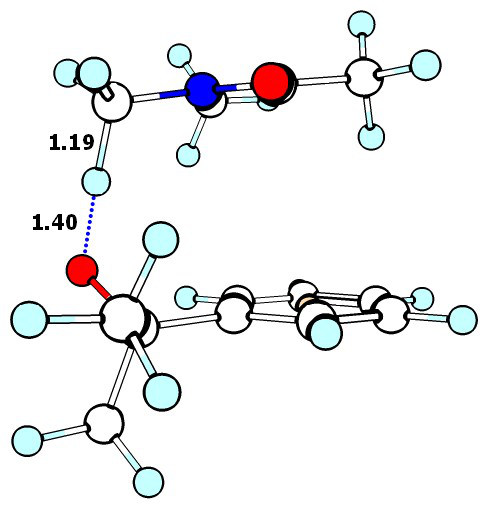
\includegraphics[width=5cm]{figures/dma-cumo-cis}
  }
  \subfigure[Cis DMA-NaCl + \cumo]{
		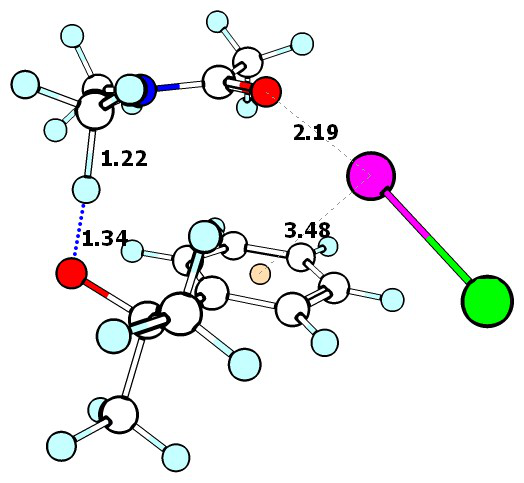
\includegraphics[width=5cm]{figures/dma-nacl-cumo-cis}
	}
  \caption[]{Continued on following page.}
\end{figure}

\begin{figure}[!htbp]\ContinuedFloat
  \setcounter{subfigure}{4}
  \subfigure[Acetyl DMA + \cumo]{
    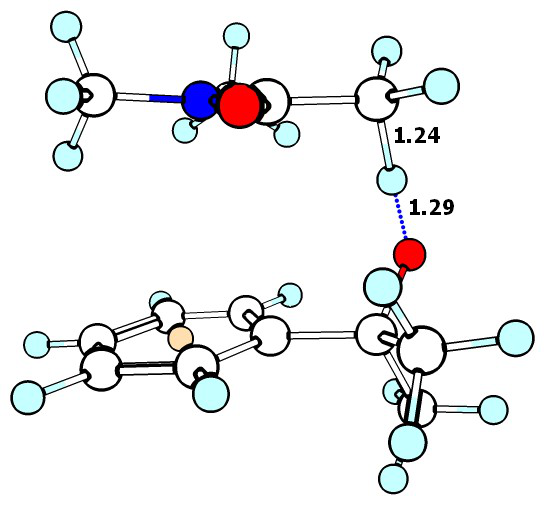
\includegraphics[width=5cm]{figures/dma-cumo-acetyl}
  }
  \subfigure[Acetyl DMA-NaCl + \cumo]{
    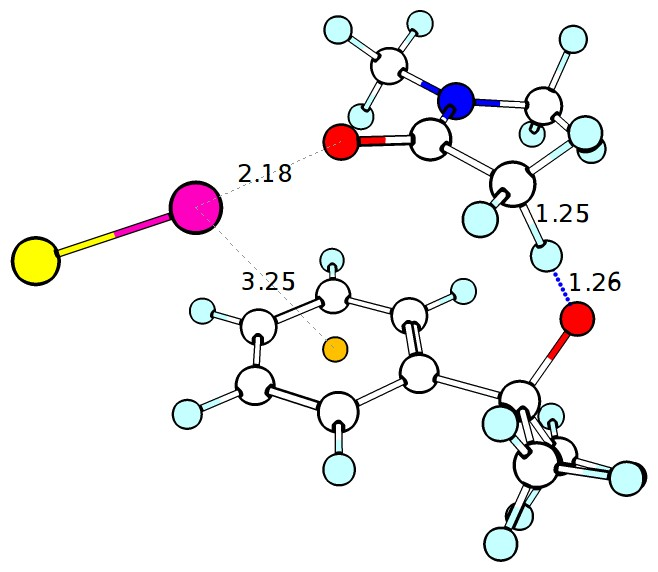
\includegraphics[width=5cm]{figures/dma-nacl-cumo-acetyl}
  }

  \caption[TS structures of HAT reaction between DMA and \cumo\ including and
  excluding NaCl.]{TS structures of HAT reaction between DMA and \cumo\
  including NaCl for different \ch{C-H} bonds: \textbf{a} trans, \textbf{b}
  trans with NaCl, \textbf{c} cis, \textbf{d} cis with NaCl, \textbf{e} acetyl,
  and \textbf{f} acetyl with NaCl. Key interatomic distances are shown in units
  of \AA. Element colour key: white is carbon, light blue is hydrogen, red is
  oxygen, blue is nitrogen, purple is sodium, green is chlorine, and peach is a
  dummy atom in the centre of an aromatic ring.}
  \label{fig:dma-cumo-ts}
\end{figure}

First, note for all the TS structures in \ref{fig:dma-cumo-ts}, the complexation
of \ch{NaCl} results in a shortening of the \ch{O-H} bond that is being formed
as a result of the HAT reaction. This indicates that the TS structure shifts
towards the product side along the reaction coordinate as a results of
interactions with \ch{NaCl}. By Hammond's postulate,\cite{Hammond1955} this
indicates a more endothermic reaction, giving evidence for increased reaction
barrier heights.

For the TS structure representing abstraction from the trans position (relative
to the carbonyl) \ch{C-H} bond of DMA by \cumo\ (\ref{fig:dma-cumo-ts}a), there
is a calculated 0.3 \kcalmol\ increase in $\Delta H^\ddagger$, which is somewhat
less than the predicted increase in BDE of 1.0 \kcalmol. This result is
consistent with the BEP principle, as the change is $\Delta H^\ddagger$ is
necessarily less than or equal to the change in $\Delta H$ due to the constant
$\alpha$ in Equation~\ref{eq:bep}. This difference can possibly be ascribed to
the effect of charge transfer: NPA indicates a 0.04 $e^-$ transfer from DMA to
\ch{NaCl}. As a result, there is less electron density available for
hyperconjugative donation to the \ch{C-H} $\sigma^*$ orbital, and thus there is
a lesser effect upon $\Delta H^\ddagger$.  Furthermore, TSs for HAT between
\ch{C-H} bond and oxygen-centred radicals are characterized by a degree of
charge separation.\cite{Roberts1999} NPA indicates that in the trans position TS
structure excluding \ch{NaCl} the charge transfer from DMA to \cumo\ is 0.24
$e^-$, but the charge transfer increases with the inclusion of \ch{NaCl} to 0.26
$e^-$. This increased charge separation results in a lower enthalpic barrier
than expected solely on the basis of the increase in \ch{C-H} BDE. While orbital
analysis does not indicate any PCET type orbital interactions, charge separation
between DMA and \cumo\ in the TS structure may be considered as a partial
ionization of the hydrogen atom. Therefore, by increasing charge separation in
the TS structure, it becomes easier to abstract the hydrogen atom as there is an
increase in the proton-transfer like character of the hydrogen atom. The
increase in $\Delta G^\ddagger$ is 3.0 \kcalmol, therefore the complexation of
metal cations increases the entropic penalty in forming the TS structure.

In the abstraction at the cis position \ch{C-H} bond of DMA by \cumo, there is a
calculated 2.6 \kcalmol\ decrease in $\Delta H^\ddagger$ and an increase of 0.9
\kcalmol\ in $\Delta G^\ddagger$. The decrease in enthalpic barrier is
inconsistent with the predicted increase in BDE of 1.8 \kcalmol\ upon
complexation with \ch{NaCl}. The TS structure in~\ref{fig:dma-cumo-ts}c shows a
possible long range interaction between \ch{Na} and the aromatic ring of \cumo\
that draws electron density and increases the reactivity. Additionally, NPA
predicts a 0.07 $e^-$ charge transfer between DMA and \ch{Na}. The combination
of these two factors stabilizes the TS and decreases $\Delta H^\ddagger$. The
entropic penalty associated with complexation of \ch{NaCl} results in an
increase in the free energy barrier.

Abstraction by \cumo\ from the acetyl \ch{C-H} bond of DMA was previously
described as being a minor reaction pathway.\cite{Salamone2013} In light of the
reduction in BDE at the acetyl position of amides, it may be reasonable to
expect the reaction barrier to decrease. This indeed appears to be the net
effect of complexation of \ch{NaCl} to DMA, as $\Delta H^\ddagger$ decreases by
3.1 \kcalmol\ and $\Delta G^\ddagger$ decreases by 0.6 \kcalmol.
\ref{fig:dma-cumo-ts}f shows that in the TS structure, \ch{Na} interacts with
the aromatic system of \cumo, which also stabilizes the TS and decreases the
barrier, but not enough to make it the lowest barrier.

For HAT between DMA and \bno, the interaction between \ch{NaCl} and \bno, are
stronger as compared to \cumo, as indicated by to the shorter distance between
\ch{Na} and the centre of the aromatic ring, as shown
in~\ref{fig:dma-bno-ts}a-f. Note that, as in reactions with \cumo, the \ch{O-H}
partial bond in the TS structures are shorter upon complexation with \ch{NaCl},
indicating greater product-like character in the TS complex. This shorter
distance is likely possible due to the easier rotation of DMA relative to \bno,
as compared to \cumo. As a result, the enthalpic barriers for the abstraction
from DMA by \bno\ decrease upon complexation of \ch{NaCl} to both the acetyl and
trans position \ch{C-H} bonds. For the cis position \ch{C-H} bond of DMA
however, the enthalpic barrier increases.

This can be explained on the basis of the presence of an interaction between
\ch{Cl} and the $\alpha$-\ch{C-H} bond of \bno. While \ch{Na} withdraws electron
density from the aromatic system of \bno, \ch{Cl} is able to donate electron
density back to \bno, counteracting the effect of the interaction of \ch{Na}.
Charge analysis confirms this, such that the NPA charge on Cl in the cis
position abstraction TS complex is -0.88 $e^-$, as compared to -0.91 $e^-$ in
abstraction from the trans position. As a result, the enthalpic barrier
increases as predicted on the basis of the increase of the cis position \ch{C-H}
BDE of DMA.

\begin{figure}[!htbp]
  \setcounter{subfigure}{0}
  \centering
  \subfigure[Trans DMA + \bno]{
		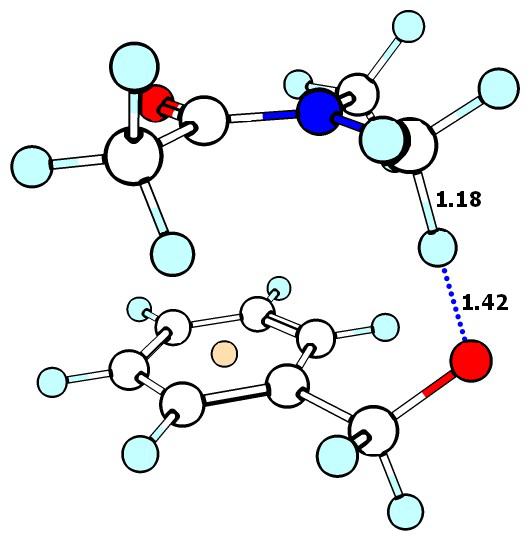
\includegraphics[width=5cm]{figures/dma-bno-trans}
	}
  \subfigure[Trans DMA-NaCl + \bno]{
		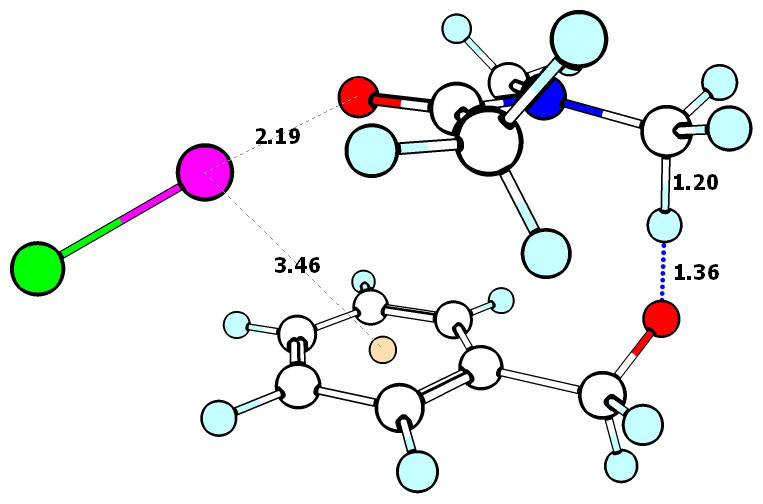
\includegraphics[width=5cm]{figures/dma-nacl-bno-trans}
	}

  \subfigure[Cis DMA+ \bno]{
		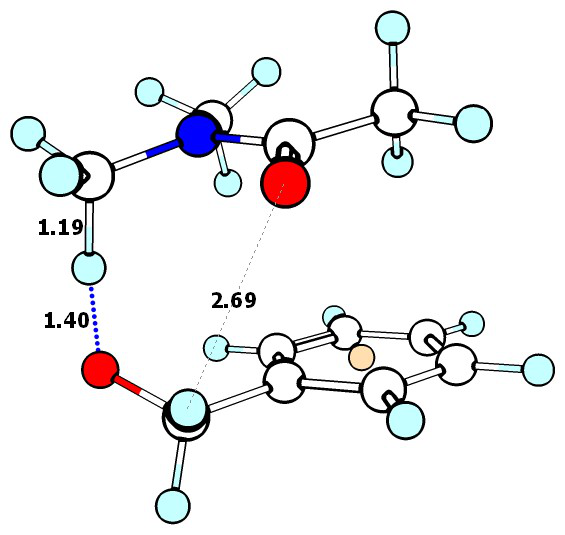
\includegraphics[width=5cm]{figures/dma-bno-cis}
	}
  \subfigure[Cis DMA-NaCl + \bno]{
		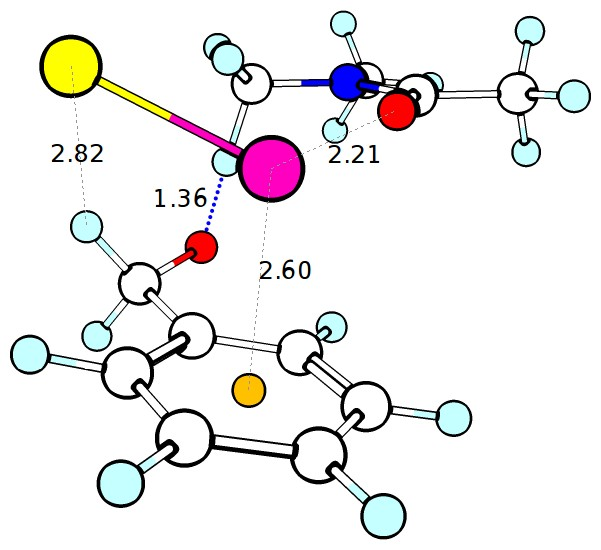
\includegraphics[width=5cm]{figures/dma-nacl-bno-cis}
	}
  \caption[]{Continued on following page.}
\end{figure}

\begin{figure}[!htbp]\ContinuedFloat
  \setcounter{subfigure}{4}
  \subfigure[Acetyl DMA + \bno]{
    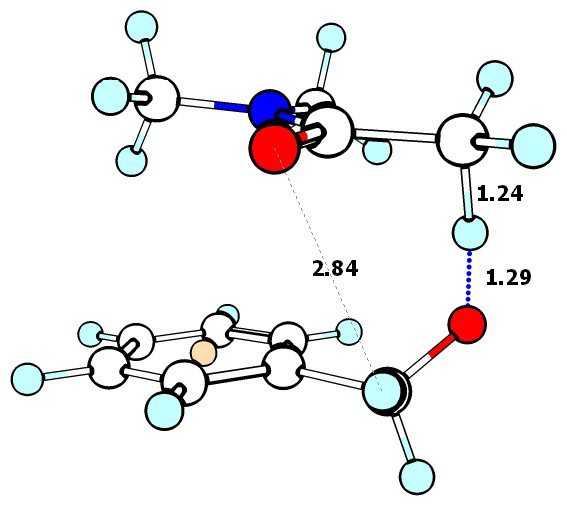
\includegraphics[width=5cm]{figures/dma-bno-acetyl}
  }
  \subfigure[Acetyl DMA-NaCl + \bno]{
    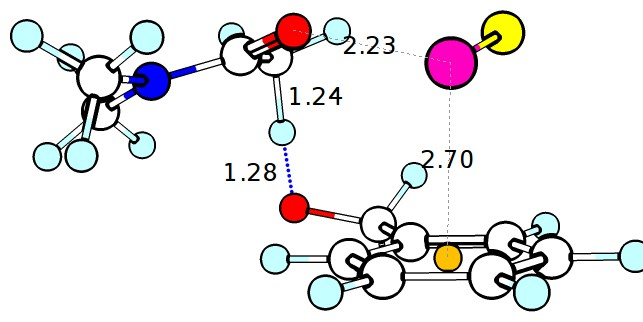
\includegraphics[width=5cm]{figures/dma-nacl-bno-acetyl}
  }

  \caption[TS structures of HAT reaction between DMA and \bno\ including
  NaCl.]{TS structures of HAT reaction between DMA and \bno\ including NaCl for
  different \ch{C-H} bonds: \textbf{a} trans, \textbf{b} trans with NaCl,
  \textbf{c} cis, \textbf{d} cis with NaCl, \textbf{e} acetyl, and \textbf{f}
  acetyl with NaCl. Key interatomic distances are shown in units of \AA.
  Element colour key: white is carbon, light blue is hydrogen, red is oxygen,
  blue is nitrogen, purple is sodium, green is chlorine, and peach is a dummy
  atom in the centre of an aromatic ring.} \label{fig:dma-bno-ts}
\end{figure}

For both \cumo\ and \bno, the presence of possible secondary interactions
between \ch{NaCl} and the radicals obfuscates the results. Therefore, in order
to determine if non-redox active metal cations may act as chemo-protective
agents in biological systems, I have performed calculation involving the more
biologically relevant \ch{HO^.} radical. Although there is no literature value
for $k_H$ of the HAT reaction between DMA and \ch{HO^.}, I have used the
Snelgrove-Ingold equation\cite{Snelgrove2001} to estimate the rate constant as
1.5\E{10} \Ms, which is two and five orders of magnitude greater than \bno\ and
\cumo, respectively. Unfortunately, I was unsuccessful in performing full
optimization calculations in the presence of the metal salt. Therefore, I have
listed these preliminary results and the analysis thereof in
Appendix~\ref{ap:hat}.


\subsection{DIA}

Next, to study the effect steric bulk has on the HAT reactions between amides
and oxygen-centred radical, I have performed a study of HAT between DIA and
\cumo. The HAT reaction between DIA and \cumo\ was previously studied by
\citet{Salamone2014}, however only the $\alpha$-N-alkyl positions were studied
theoretically. Since the BDEs for $\alpha$- and $\beta$-N-alkyl \ch{C-H}
positions are relatively close in energy, I calculated the reaction barriers
for these positions as well. The calculated free energy (enthalpic) barriers
excluding and including \ch{NaCl} are listed in ~\ref{tab:dia-cumo}.
Interestingly the predicted reaction barriers for abstraction of the
$\beta$-positions of DIA are lower than the $\alpha$-positions. By applying the
Boltzmann distribution about 69\% of abstractions by \cumo\ from DIA will take
place from either the cis- or trans-$\beta$ positions of DIA. Therefore,
abstraction from bulky amides by bulky oxygen-centred radicals are likely
controlled by steric considerations. Note also that many of the TS
optimizations were not successful with the inclusion of \ch{NaCl} and in which
case ``guess'' TS structures have been used to estimate the barrier heights.
The TS structures for the HAT reaction between DIA and \cumo\ including
\ch{NaCl} are shown in~\ref{fig:dia-cumo-ts}.

\begin{table}[!htbp]
\caption[Calculated free energy (enthalpy) for direct HAT from different
\ch{C-H} bonds in DIA by \cumo, with and without \ch{NaCl}.]{Calculated free
energy (enthalpy) ($\Delta G(H)^\ddagger$, \kcalmol) for direct HAT from
different \ch{C-H} bonds in DIA by \cumo, with and without \ch{NaCl}. The change
in barrier height ($\Delta \Delta G(H)^\ddagger$) is calculated relative to the
same abstraction site without the inclusion of \ch{NaCl}. All barrier heights
are relative to separated reactants (or complexed DIA-NaCl) and were calculated
at the M05-2X-SMD(MeCN)/6-311+G(2d,2p)//M05-2X/6-31+G$^{**}$ level of theory.
$^*$Indicates estimated barrier based on ``guess'' TS structure.}
\label{tab:dia-cumo}
  \begin{tabular}{l l c c}
    Reaction   &  Abstraction Site   &  $\Delta G(H)^\ddagger$ &  $\Delta \Delta G(H)^\ddagger$ \\
    \hline
    DIA + \cumo    &  $\alpha$-trans    &  19.5(6.2)  &              \\
                   &  $\alpha$-cis      &  19.1(5.4)  &              \\
                   &  $\beta$-trans     &  18.6(6.0)  &              \\
                   &  $\beta$-cis       &  18.4(6.5)  &              \\
                   &  acetyl         &  19.1(7.4)  &              \\
    DIA-NaCl + \cumo &  $\alpha$-trans$^*$  &  17.0(3.9)  &   -2.5(-2.3)  \\
                   &  $\alpha$-cis$^*$      &  12.7(-2.4) &   -6.4(-7.8) \\
                   &  $\beta$-trans     &  19.8(6.8)  &    0.7(1.4)  \\
                   &  $\beta$-trans$^*$     &  19.6(6.9)  &    0.5(1.5)  \\
                   &  $\beta$-cis$^*$       &  16.8(4.2)  &   -1.6(-2.3) \\
                   &  acetyl$^*$         &  17.8(3.8)  &    0.8(-0.1) \\
                   &  acetyl             &  17.9(3.7)  &    0.9(-0.2)
  \end{tabular}
\end{table}

\begin{figure}
  \setcounter{subfigure}{0}
  \centering

  \subfigure[$\alpha-$trans DIA-NaCl + \cumo]{
		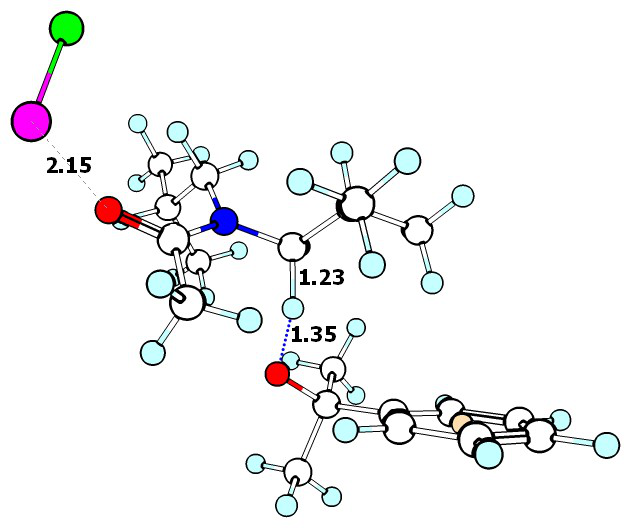
\includegraphics[width=5cm]{figures/dia-nacl-cumo-trans-alpha}
	}
  \subfigure[$\alpha-$cis DIA-NaCl + \cumo]{
		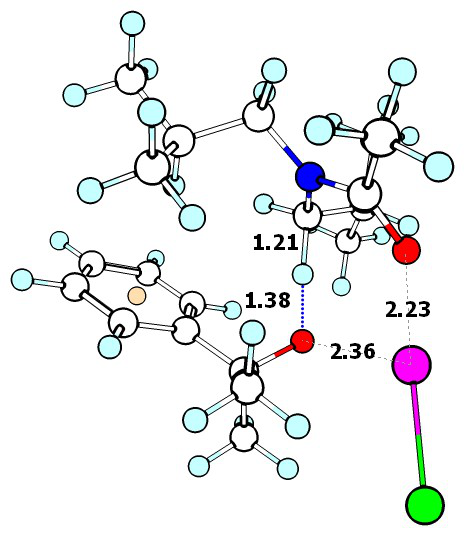
\includegraphics[width=5cm]{figures/dia-nacl-cumo-cis-alpha}
	}

  \subfigure[$\beta-$trans DIA-NaCl + \cumo]{
		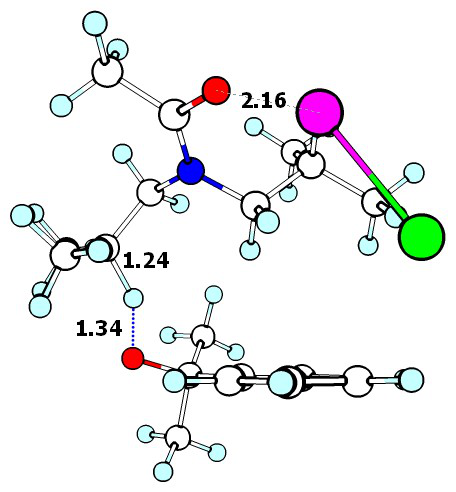
\includegraphics[width=5cm]{figures/dia-nacl-cumo-trans-beta}
	}
  \subfigure[$\beta-$cis DIA-NaCl + \cumo]{
		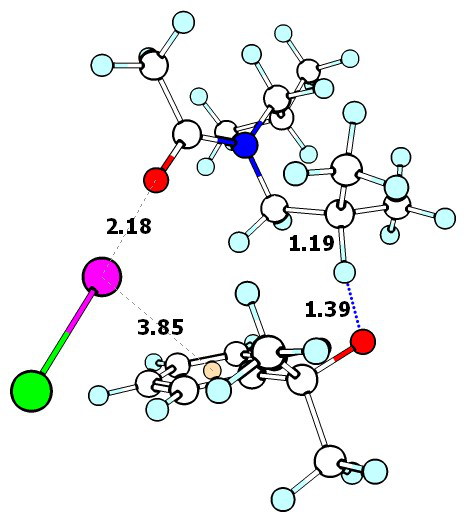
\includegraphics[width=5cm]{figures/dia-nacl-cumo-cis-beta}
	}
  \caption[]{Continued on following page.}
\end{figure}

\begin{figure}\ContinuedFloat
  \setcounter{subfigure}{4}
  \subfigure[Acetyl DIA-NaCl + \cumo]{
    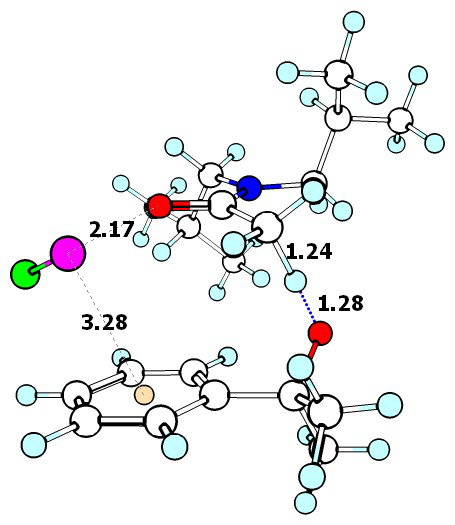
\includegraphics[width=5cm]{figures/dia-nacl-bno-acetyl}
  }

  \caption[TS structures for HAT reaction between DIA and \cumo\ including
  NaCl.]{TS structures for HAT reactions between DIA and \cumo\ including NaCl
  for different \ch{C-H} bonds: \textbf{a} $\alpha$-trans, \textbf{b}
  $\alpha$-cis, \textbf{c} $\beta$-trans, \textbf{d} $\beta$-cis, and
  \textbf{e} acetyl. Key interatomic distances are shown in units of \AA.
  Element colour key: white is carbon, light blue is hydrogen, red is oxygen,
  blue is nitrogen, purple is sodium, green is chlorine, and peach is a dummy
  atom in the centre of an aromatic ring.}
  \label{fig:dia-cumo-ts}
\end{figure}

As was observed in the barrier height calculations involving \ch{NaCl} with DMA
with \bno\ and \cumo, the results vary depending on the presence or absence of
secondary interactions of \ch{Na} with \cumo. For the $\beta$-cis and acetyl
position of DIA (\ref{fig:dia-cumo-ts}d-e), $\Delta H^\ddagger$ decreases by 2.3
and 0.2 \kcalmol, respectively, as a result of relatively long range
interactions of \ch{Na} with the aromatic system of \cumo. For abstraction from
the $\alpha$-cis position of DIA (\ref{fig:dia-cumo-ts}b), \ch{Na} is able to
interact with both the amidic oxygen lone pair, and a lone pair on the oxygen of
\cumo, resulting in a significant decrease in $\Delta H^\ddagger$ by 7.8
\kcalmol.

For the $\alpha$-trans position there is no interaction between \ch{Na} and
\cumo, however the complexation of \ch{NaCl} to DIA results in a 2.5 \kcalmol\
decrease in $\Delta G^\ddagger$. Comparing the TS structures including and
excluding NaCl, there is very little difference. Therefore, it is likely that
the ``guess'' TS structure including NaCl does not appropriately represent the
``true'' TS structure for this particular abstraction site. Note that this may
also be the case in other systems.

Abstraction by \cumo\ from the $\beta$-trans position of DIA does not allow for
an interaction between both the amidic oxygen and \cumo. However, there should
be no effect from decreased electron density in the \ch{C-H} $\sigma^*$ orbital.
Consequently, $\Delta H^\ddagger$ increases by 1.4 \kcalmol\ as a result of the
effect of 0.04 $e^-$ charge transfer from DIA to \ch{Na} in the TS structure.


\section{Summary}

In this investigation, the effects of non-redox active metal cations upon the
barrier heights of HAT reactions between small models for proteins with
oxygen-centred radicals were studied. I began by examining the effects of the
complexation of \ch{NaCl} upon the \ch{C-H} bond strengths of the substrates of
interest in this work. This in particular is central to the hypothesis of this
work: complexation of a non-redox active metal to a heteroatom of a substrate
reduces the electron density donated to adjacent \ch{C-H} $\sigma^*$ orbitals,
increasing the \ch{C-H} bond strength. By the BEP principle (See
Chapter~\ref{ch:bde}), the HAT reaction barrier height increases as a function
of the \ch{C-H} BDE.

Specific metal-substrate interactions can increase the effective \ch{C-H} BDEs
in the parent molecule, however this is complicated by the possibility for
metal-radical interactions following bond cleavage. Metal-radical interaction
can either increase or decrease \ch{C-H} BDEs depending on the nature of the
orbital interactions of the product radical and metal cation. The aforementioned
hypothesis does not take into account the effects of metal-radical interaction.

Next, I studied the effects of metal complexation on the HAT reaction barrier
heights. I calculated the barrier heights for two small models for proteins, DMA
and DIA, including and excluding \ch{NaCl}, with two different oxygen-centred
radical, \bno\ and \cumo. In the absence of any secondary interactions in the TS
complex, the enthalpic HAT reaction barrier increases as a results of metal
complexation. However, in the event of interactions between either the sodium or
chlorine moieties with the oxygen-centred radical or extensions of the substrate
in the TS complex, the effect of complexation can increase or decrease the
barrier height, depending on the specific interaction. This further motivates
the idea that the central hypothesis is incomplete in describing the effects of
non-redox active metals on HAT reaction barrier heights.

The results obtained herein do not align with those from experiment. Recall that
previous experimental results for the HAT reaction between DMA and \cumo\
demonstrated clear inhibition upon the addition of alkali and alkaline
earth-metal salts. There are several possible explanations for this discrepancy:
The models used herein may not properly capture the behaviour of bulk systems
with respect to solvation or stoichiometry (the binding of multiple amide
substrates to a single metal cation). Another possible explanation is the use of
\ch{Cl^-} as a counteranion herein, whereas \ch{ClO4^-} and \ch{OTf^-} were
utilized in experiment; the nature of the counteranion may play a larger roll
than has been previously demonstrated.

The sum of these results suggests that non-redox active metal cations may not
always deactivate \ch{C-H} bonds in complex chemical environments. Therefore, on
the basis of these limited results, it seems unlikely that a natural
chemo-protective effect is observed due to the presence of alkali and alkaline
earth-metal cations in protein or other biological systems. Additional work
should be carried out to corroborate these results.


\end{doublespace}
